\documentclass[12pt,a4paper]{report}
\usepackage{ragged2e}
\usepackage[utf8]{inputenc}
\usepackage[english]{babel}
\usepackage{fancyvrb}
\usepackage{multirow}
\usepackage{rotating}
\usepackage{slashbox,pict2e}
\usepackage{soul}
\usepackage{amssymb}
\usepackage{lscape}
\usepackage{longtable}
\usepackage{makeidx}
\usepackage{amsmath}
\usepackage{multirow}
\usepackage{makecell}
\usepackage{wrapfig}
\usepackage{graphicx}
\usepackage{float}
\usepackage[caption = false]{subfig}
\setcounter{secnumdepth}{4} 
\setcounter{tocdepth}{6}
\usepackage[utf8]{inputenc}
\usepackage[left=3cm, right=3cm, top=3cm, bottom=3cm]{geometry}
\graphicspath{{Figures/}}
\justifying
\usepackage{ragged2e}
\begin{document}

\pagenumbering{roman}

\title{
\includegraphics[width=0.5\textwidth]{AU-Logo.png}\\}

\author{
	Usama Rao \\ 161120 \and
	
	Sami Ahmed \\ 161132  \and
	
	\\\\
	
	\textbf{\Large CarPool}
	
	\\\\\\
	
	\textbf{\large Bachelor of Science in Computer Science}
	
	\\\\
	
	{\normalsize Supervisor: Shoaib Malik}
	
	\\\\
	
	{\normalsize Co-Supervisor: Dr. Tauseef}
	
	\\\\
	
	{\normalsize Department of Computer Science}
	
	\\\\
	
	{\normalsize Air University, Islamabad}
	
	\date{\normalsize June 2020}
}

\maketitle

\thispagestyle{empty}

\cleardoublepage

\newpage 

\thispagestyle{empty}

\vspace*{0.9\textheight}

\begin{center}
	
	Copyrights \copyright Usama Rao and Sami Ahmed, 2020
	
\end{center}

\newpage

\thispagestyle{empty}

\begin{center}
	
	\section*{\Huge Certificate}
	
\end{center}

\vspace*{0.1\textheight}

{We accept the work contained in the report titled 'CarPool', written by Mr. Usama Rao  AND Mr. Sami Ahmed as a confirmation to the required standard for the partial fulfillment of the degree of Bachelor of Science in Computer Science.}

\vspace*{0.1\textheight}

Approved by...:\\

Supervisor:\\

\hspace{2cm}\hrulefill

\bigskip 

Internal Examiner: \\

\hspace{2cm}\hrulefill

\bigskip 

External Examiner: \\

\hspace{2cm}\hrulefill

\bigskip 

Project Coordinator: \\

\hspace{2cm}\hrulefill

\bigskip 

Head of the Department: \\

\hspace{2cm}\hrulefill

\bigskip 

\vspace*{0.1\textheight}

June, 2020

\newpage

\thispagestyle{empty}

\mbox{}

\newpage

\renewcommand*\contentsname{Table of Contents}

\tableofcontents

\renewcommand{\listfigurename}{List of Figures}

\listoffigures

\chapter*{Abstract}
\addcontentsline{toc}{chapter}{Abstract}
In general, people have a hard time conciliating their schedules because of the way they move from one location to another.  and students suffer from this the most  especially  since transportation between cities is not that great,  As students, we think there should exist more suitable transportation solutions to places where transportation networks are short and cheap and helpful for students.
\\ This  report  proposes  a  platform  to  help  improve students  mobility  through carpooling, a way for vehicle owning students to share their private vehicle with non vehicle owning students in order to splitting and reducing costs. carpooling may be one of the best solutions when there is no other  mean  of  transportation  to a  specific location  but naturally  it  is not  the  only one. mobile applications  take more  and more  part of  everyone’s  lives, different  services for carpooling with different features begin to compete with existing transportation solutions. some people start to  prefer using  new carpooling  services  over the  traditional services represented  by  taxi  services. carPool  aims  to  promote  carpooling  by  targeting  students making it easier for them to adhere and use this system.  by  targeting  students  people  will  more  likely  join  the  service  since  its  users  are primarily other people form the same environment. to put the carpooling system in place, we have designed and developed an android mobile application with backend servers for users  to  access  the  carpooling  service  through  their  smartphones,  additionally  the application  involves  some  features  that  are  critical  to  the  service.  by  using  android development  tools  and  libraries and  efficient backend  solutions  we  have managed  to make the application simple but powerful as well, which makes this application very useful for the students to use.
\\ The combination of the smart phone and the internet service is the trend of the future information development and software applications. mobile phones are the most commonly used communication tools. using mobile phones to obtain information is not only quick, but also more convenient shortcut to improve people's lives. in the paper, we propose the software development architecture based on web services. this framework introduces the three-layer architecture of web development into mobile phone software development. based on the threelayer architecture, the android based carPool system is developed.
\\ Our app CarPool will be a unique carpooling application that would take benefits of the advantages of carpooling and try to improve and eliminate the disadvantages, all while focusing on making it a good carpooling experience for students. the realization of our project will go through the conceptual phase and then development phase. since making a good application requires good planning first.
\chapter*{Acknowledgments}
\addcontentsline{toc}{chapter}{Acknowledgments}

We wish to thank various people for their contribution to this project. We would like to express our deep gratitude to Sir Shoaib Malik, our Project supervisor, for their patient guidance, enthusiastic encouragement and useful critiques of this project work. We would also like to thank Dr. Touseef Javed, our project co-supervisor for his advice and assistance in keeping our progress on schedule. We would also like to extend our thanks to the librarians of the Air University for their help in offering us the resources in running the program.\\

Finally, we wish to thanks our parents for their support and encouragement throughout our study.


\vspace{10mm}


\flushleft{\textsc{Usama, Sami Ahmed Malik}\\Islamabad, Pakistan}

\flushleft{June 2020}

\pagenumbering{arabic}
\chapter{Introduction} \label{chap:intro}

\section*{What is CarPool?}

\section{Project Background/Review}
\justify
Carpooling (also car-sharing, ride-sharing and lift-sharing) is the sharing of car journeys so that more than one person travels in a car, and prevents the need for others to have to drive to a location themselves.
\\ Drivers and passengers offer and search for journeys through one of the several mediums available. after finding a match they contact each other to arrange any details for the journey(s). Costs, meeting points and other details like space for luggage are agreed on. They then meet and carry out their shared car journey(s) as planned.
\\ By having more people using one vehicle, carpooling reduces each person's travel costs such fuel costs, tolls and the stress of driving. authorities often encourage carpooling, especially during periods of high pollution or high fuel prices. car sharing is a good way to use up the full seating capacity of a car, which would otherwise remain unused if it were just the driver using the car.
\\ In 2009, carpooling represented 43.5\% of all trips in the United States and 10\% of commute trips. The majority of carpool commutes (over 60\%) are "fam-pools" with family members.
in 2011, an organization called Greenock created a campaign to encourage others to use this form of transportation in order to reduce their own carbon footprint.
\\ Carpooling, or car sharing as it is called in British English, is promoted by a national UK charity, Carplus, whose mission is to promote responsible car use in order to alleviate financial, environmental and social costs of motoring today, and encourage new approaches to car dependency in the UK. carplus is supported by transport for London, the British government initiative to reduce congestion and parking pressure and contribute to relieving the burden on the environment and to the reduction of traffic related air-pollution.
\\ Cabbing All the Way is a book written by author Jatin Kuberkar that narrates a success story of a carpool with twelve people on board. based in the city of Hyderabad, India, the book is a real-life narration and highlights the potential benefits of having a carpool

\section{Problem description}
Many vehicle-owning Students who commute on daily basis often have unoccupied seats in their vehicles. many non-vehicle owning students find it very difficult sometimes to find ride for travelling to and from university.

\section{Project Objectives}
\textbf{Objective}
\begin{itemize}

\item To Allow vehicle owning students to share their rides with other students for traveling to and from their institutes and cut down their fuel bills.

\item To facilitate non-vehicle owning students for travelling to and from university easier and cheaper.

\end{itemize}
\textbf{Goals}
\begin{itemize}

\item Cost Effective: much Cheaper than Cab services.
\item Ease of getting ride: riders are easy approachable, which reduces the tension of finding and catching of local transport right on time.
\item Fewer Cars on the road will have reduced fuel consumption which will make environment eco-friendly.
\end{itemize}

\section{Project Scope}
This project (CarPool) aims to develop an Android based application for carpooling for students, this application allows vehicle owning students to submit rides for specific targets and allows passengers to reserve/request rides from drivers all while being secure and having a simple interface.
\\ This application will help students save money and also reduce the pollution of the environment and effects of vehicles, this application focuses on serving needs of students. CarPool will be intended for the students in Air University and it will support android phones and tablets, users will need internet connection to use the application to offer or find a common route to travel.
\\ The application will have a simple and easy interface, Users must register at first before using the application, after that they must choose between a driver or a passenger, a driver can offer a drive to a specific location while a passenger can find or request a ride to a location.

\section{The Degree of Project Report}
In our FYP-1, we presented our idea that how CarPool would be beneficial. the only purpose of FYP-1 was to present and defend the idea. We have completed both tasks successfully and we also developed some mockup screens to present our idea.
\\ However, in fyp-2, the task assigned to us was to develop a working application for two users: driver and rider along with the implementation of the core feature of our application, which was location tracking of driver and rider, fetching current location, use Firebase it’s real-time database which is a NoSQL fast databaseand displaying that location on the map using Google Map API.
 
\chapter{Literature Review} \label{chap:literatureReview}

\section*{Carpooling}

\section{Definition and general principle}
Carpooling (also car-sharing, ride-sharing and lift-sharing) is the sharing of car journeys       so that more than one person travels in a car, and prevents the need for others to have to drive to a location themselves.
\\ By having more people using one vehicle, carpooling reduces each person's travel costs 
such as: fuel costs, tolls, and the stress of driving. Carpooling is also a more environmentally 
friendly and sustainable way to travel as sharing journeys reduces air pollution, carbon 
emissions, traffic congestion on the roads, and the need for parking spaces. Authorities 
often encourage carpooling, especially during periods of high pollution or high fuel prices.
Car sharing is a good way to use up the full seating capacity of a car, which would otherwise 
remain unused if it were just the driver using the car.
\\ In 2009, carpooling represented 43.5\% of all trips in the United States and 10\% of 
commute trips. The majority of carpool commutes (over 60\%) are "fam-pools" with family 
members.
\\ Carpool commuting is more popular for people who work in places with more jobs 
nearby, and who live in places with higher residential densities. Carpooling is significantly 
correlated with transport operating costs, including fuel prices and commute length, and 
with measures of social capital, such as time spent with others, time spent eating and 
drinking and being unmarried. However, carpooling is significantly less likely among 
people who spend more time at work, elderly people, and homeowners. 
\\ Carpooling usually means to divide the travel expenses equally between all the 
occupants of the vehicle (driver or passenger). The driver does not try to earn money, but 
to share with several people the cost of a trip he would do anyway. The expenses to be 
divided basically include the fuel and possible tolls. But if we include in the calculation the 
depreciation of the vehicle purchase and maintenance, insurance and taxes paid by the 
driver, we get a cost around 100DA/km. There are platforms that facilitate carpooling by 
connecting people seeking respectively passengers and drivers. Usually there is a fare set 
up by the car driver and accepted by passengers because they get an agreement before trip 
start.

\section{Carpooling Types}
\subsection{Regular}
The car is often perceived as an extension of the personal space, the driver, alone in 
his vehicle is in a closed space; he is free to do what he likes: listen to the radio, sing, call 
with headsets ... Carpooling regularly is to share a dialogue, experiences, stories.
In the United States an intermediate concept has developed between carpooling and 
the public transport line: the Vanpool. These are minibuses chartered by an employer, a 
public authority or a private company and made available to a group of people who 
regularly make the same journey.

\subsection{Occasional}
This type of carpooling is mainly used for leisure or last minute departures. The 
linking is often done through websites or mobile applications, which can significantly 
reduce travel costs, but usually requires to carpool with one or more unknown.
This type of carpooling is mainly used for leisure or last minute departures. The 
linking is often done through websites or mobile applications, which can significantly 
reduce travel costs, but usually requires to carpool with one or more unknown.

\subsection{Eventual}
Participants in an event (music festival, sporting event, wedding, associative or 
institutional meeting ...) can organize to carpool to the venue of the event. This one-time 
carpool has a special feature: all participants travel to the same place on the same date.
Carpooling is also used for departures on holidays or weekends, savings on a trip 
being even larger than the trip is long. So carpooling becomes an alternative of affordable 
and accessible transportation.
\\ There are also "cultural" carpooling platforms to visit a cultural site: castles, 
museums, exhibitions, artists' studios, religious places, festivals, etc.

\chapter{Requirement Specifications} \label{chap:reqs}

\subsection{Existing System for carpooling}
\justify
Many carpoolings applications and websites have been developed around the world. a similar carpooling system was developed in Massey University New Zealand by a group of students to allow students of Massey University, Albany campus to share their vehicle with non-vehicle owning students.
\\ Following some examples of carpooling systems around the globe : 

\subsection{Websites}
\begin{itemize}

\item New Zealand: https://www.asa.ac.nz/carpool
\item Algeria: www.nroho.com, www.m3aya.com,www.nsogo.net
\item Europe: BlaBlaCar.com, carpooling.com, GoMore.com
\item France: covoiturage.fr
\item USA: car.ma , www.rdvouz.com
\item World: Outpost.travel , joinntravel.com , www.letsride.in

\end{itemize}

\subsection{Mobile Applications}
\begin{itemize}

\item New Zealand: ASA
\item Algeria: YAssir,Nsogo, AMIR
\item World: Uber, sRide, RideShare, 
\item USA: Uber, Lyft
\item France: Karos, Wever, BlaBlaCar, OuiHop

\end{itemize}
\section{Proposed System}
Our purposed system is a “Carpool” application which is a ride sharing application designed just for students.students can login or signup to this application only via university email id to make sure that only enrolled students in a university used this application.
\\ Vehicle owning students can share their rides with other students for traveling to and from their institutes and earn money.

\section{Requirement Specifications}
It involves functional and non-functional functionalities that must be performed by the system:

\subsection{Functional Requirements}

\begin{figure}[ht]
\subsubsection{Table 1: Functional Requirement - 01}
\centering
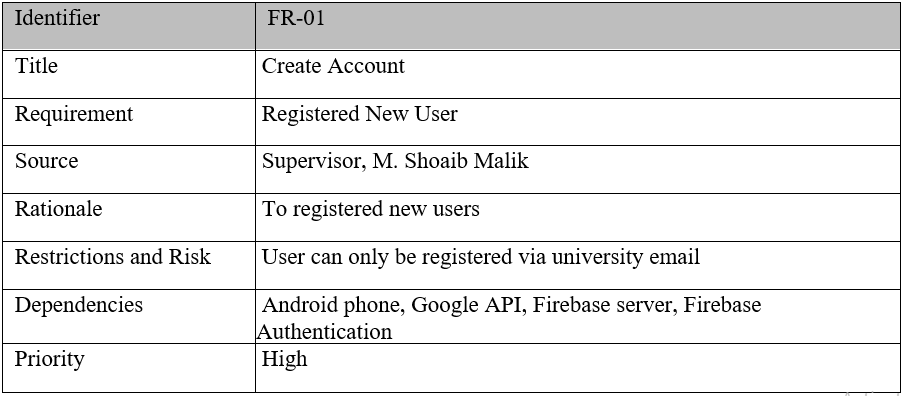
\includegraphics[width=0.8\textwidth]{TableFR1}
\end{figure}

\begin{figure}[ht]
\subsubsection{Table 2: Functional Requirement - 02}
\centering
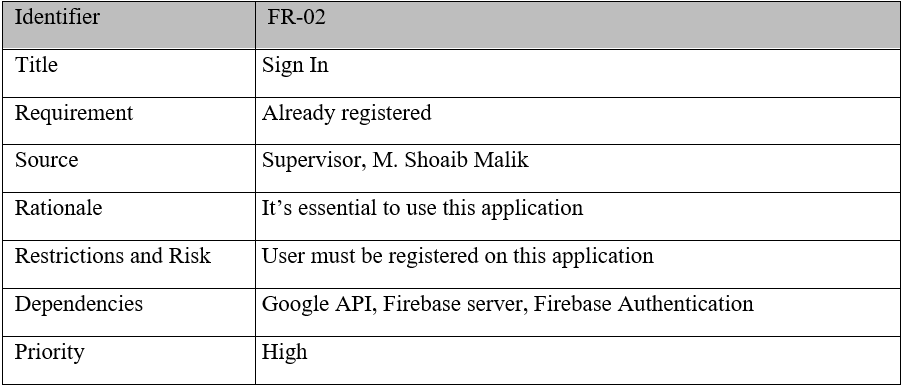
\includegraphics[width=0.8\textwidth]{TableFR2}
\end{figure}

\begin{figure}[ht]
\subsubsection{Table 3: Functional Requirement - 03}
\centering
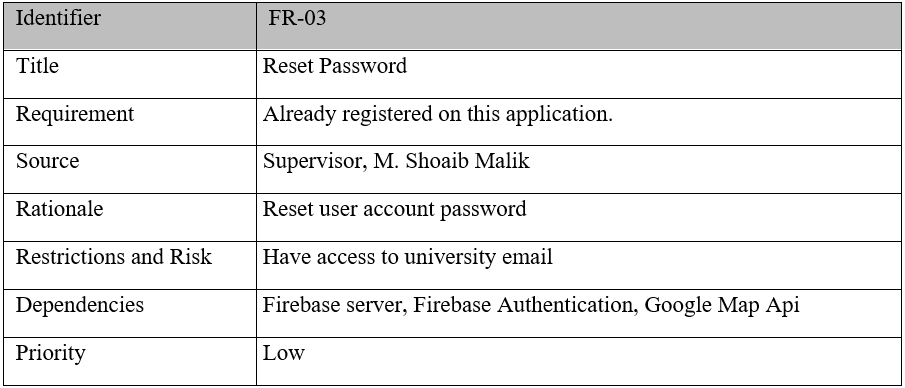
\includegraphics[width=0.8\textwidth]{TableFR3}
\end{figure}

\begin{figure}[ht]
\subsubsection{Table 4: Functional Requirement - 04}
\centering
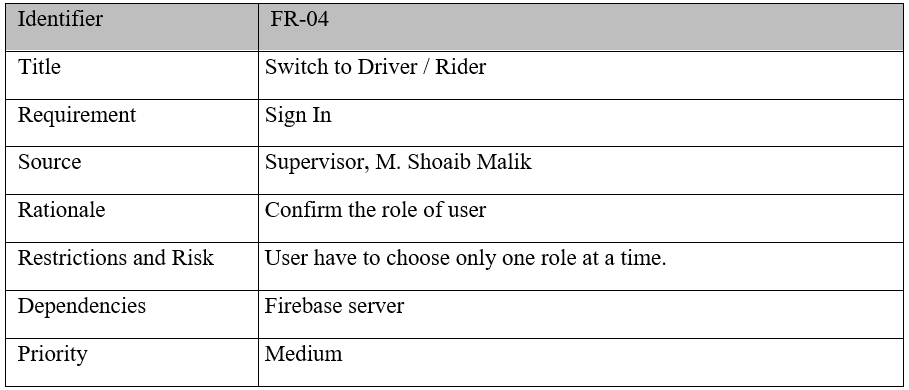
\includegraphics[width=0.8\textwidth]{TableFR4}
\end{figure}

\begin{figure}[ht]
\subsubsection{Table 5: Functional Requirement - 05}
\centering
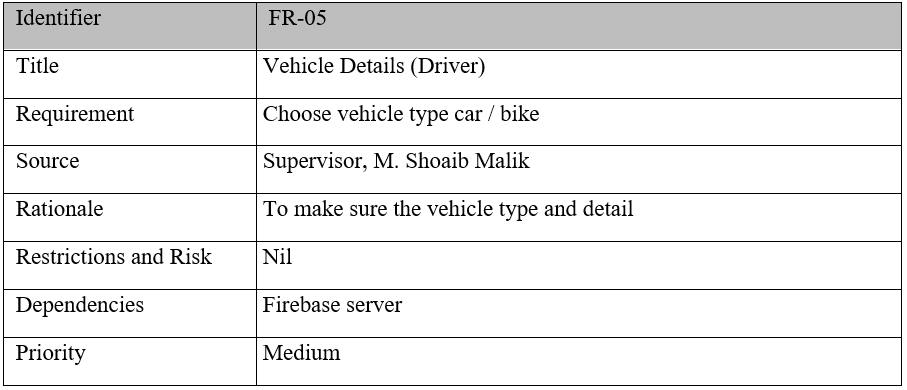
\includegraphics[width=0.8\textwidth]{TableFR5}
\end{figure}

\begin{figure}[ht]
\subsubsection{Table 6: Functional Requirement - 06}
\centering
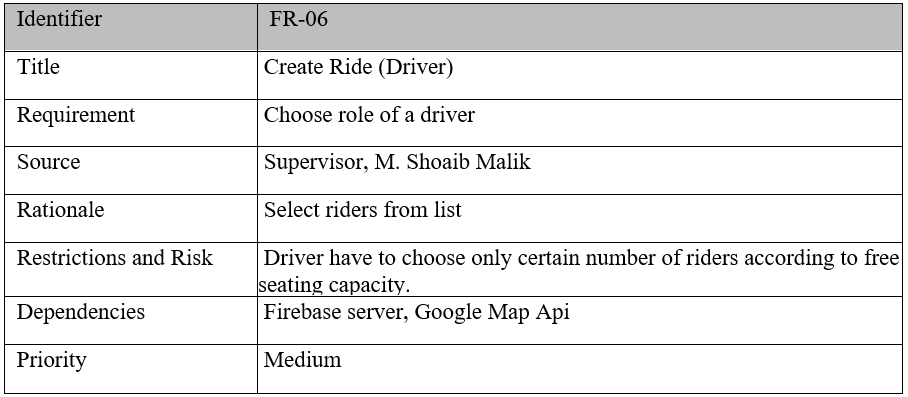
\includegraphics[width=0.8\textwidth]{TableFR6}
\end{figure}

\begin{figure}[ht]
\subsubsection{Table 7: Functional Requirement - 07}
\centering
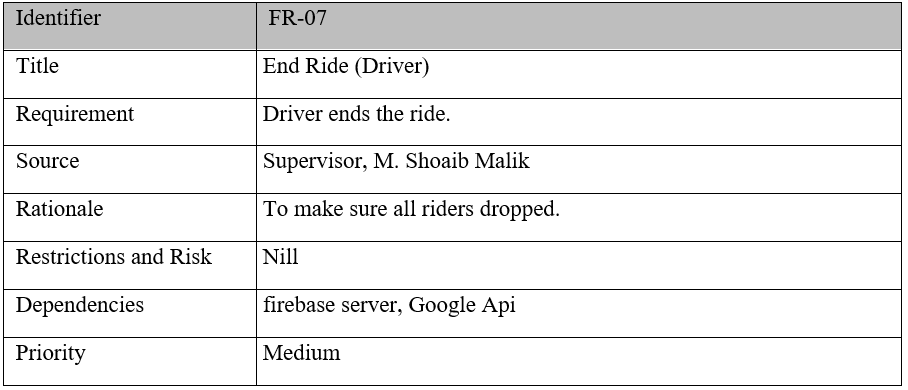
\includegraphics[width=0.8\textwidth]{TableFR7}
\end{figure}

\begin{figure}[ht]
\subsubsection{Table 8: Functional Requirement - 08}
\centering
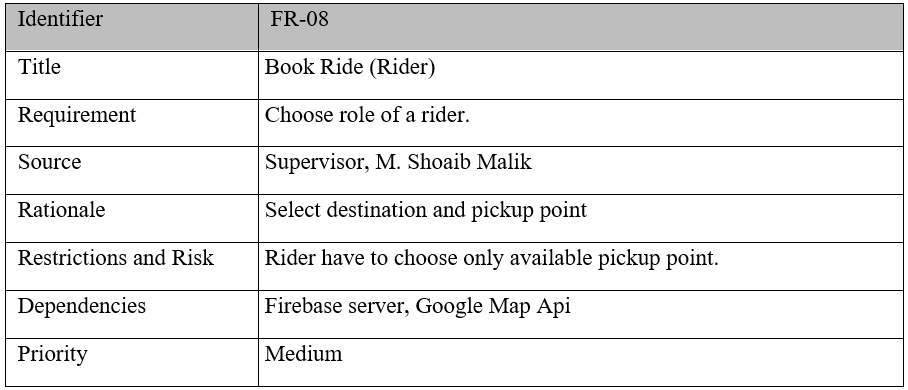
\includegraphics[width=0.8\textwidth]{TableFR8}
\end{figure}

\begin{figure}[ht]
\subsubsection{Table 9: Functional Requirement - 09}
\centering
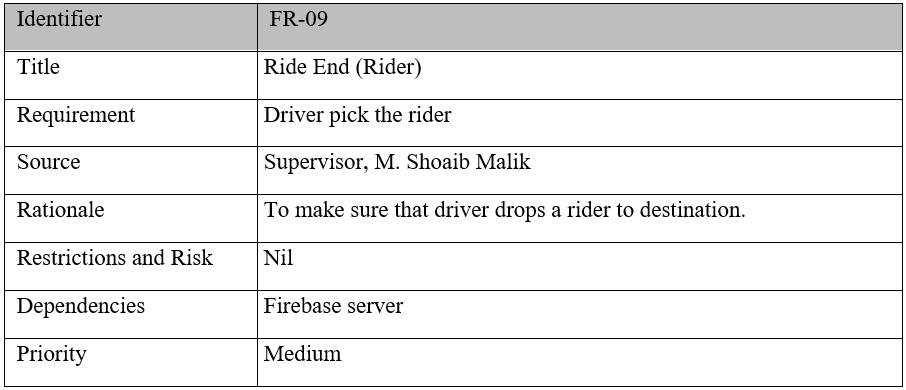
\includegraphics[width=0.8\textwidth]{TableFR9}
\end{figure}

\begin{figure}[ht]
\subsection{Non-Functional Requirements} 

\subsubsection{Table 10: Non-Functional Requirement - 01}
\centering
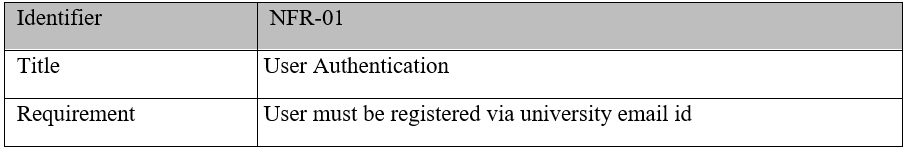
\includegraphics[width=0.8\textwidth]{TableNFR1}
\end{figure}

\begin{figure}[ht]
\subsubsection{Table 11: Non-Functional Requirement - 02}
\centering
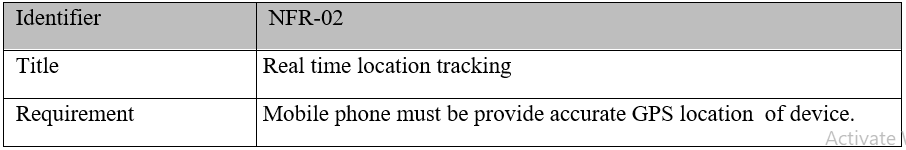
\includegraphics[width=0.8\textwidth]{TableNFR2}
\end{figure}

\begin{figure}[ht]
\subsubsection{Table 12: Non-Functional Requirement - 03}
\centering
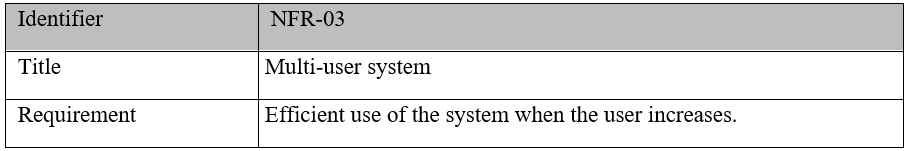
\includegraphics[width=0.8\textwidth]{TableNFR3}
\end{figure}

\begin{figure}[ht]
\subsubsection{Table 13: Non-Functional Requirement - 04}
\centering
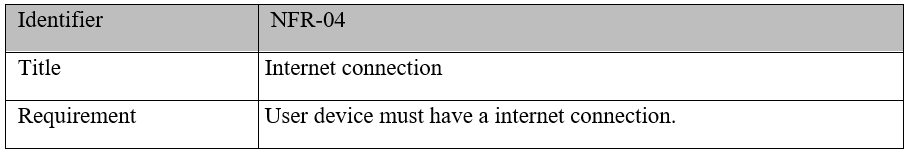
\includegraphics[width=0.8\textwidth]{TableNFR4}
\end{figure}

\begin{figure}[ht]
\subsubsection{Table 14: Non-Functional Requirement - 05}
\centering
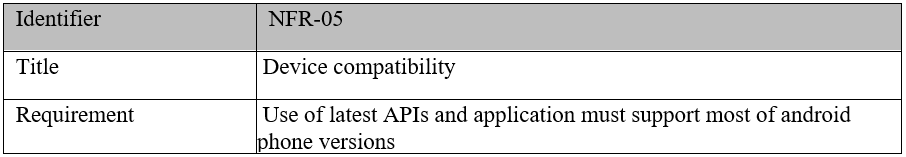
\includegraphics[width=0.8\textwidth]{TableNFR5}
\end{figure}

\begin{figure}[ht]
\subsubsection{Table 15: Non-Functional Requirement - 06}
\centering
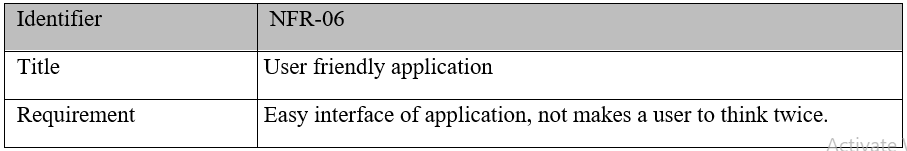
\includegraphics[width=0.8\textwidth]{TableNFR6}
\end{figure}

\begin{figure}[ht]
\subsubsection{Table 16: Non-Functional Requirement - 07}
\centering
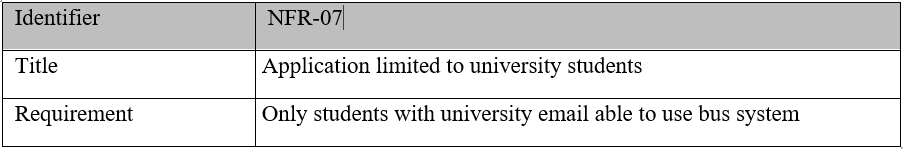
\includegraphics[width=0.8\textwidth]{TableNFR7}
\end{figure}
\begin{figure}
\section{Use Cases}
\subsection{Use Case Diagram}
\center
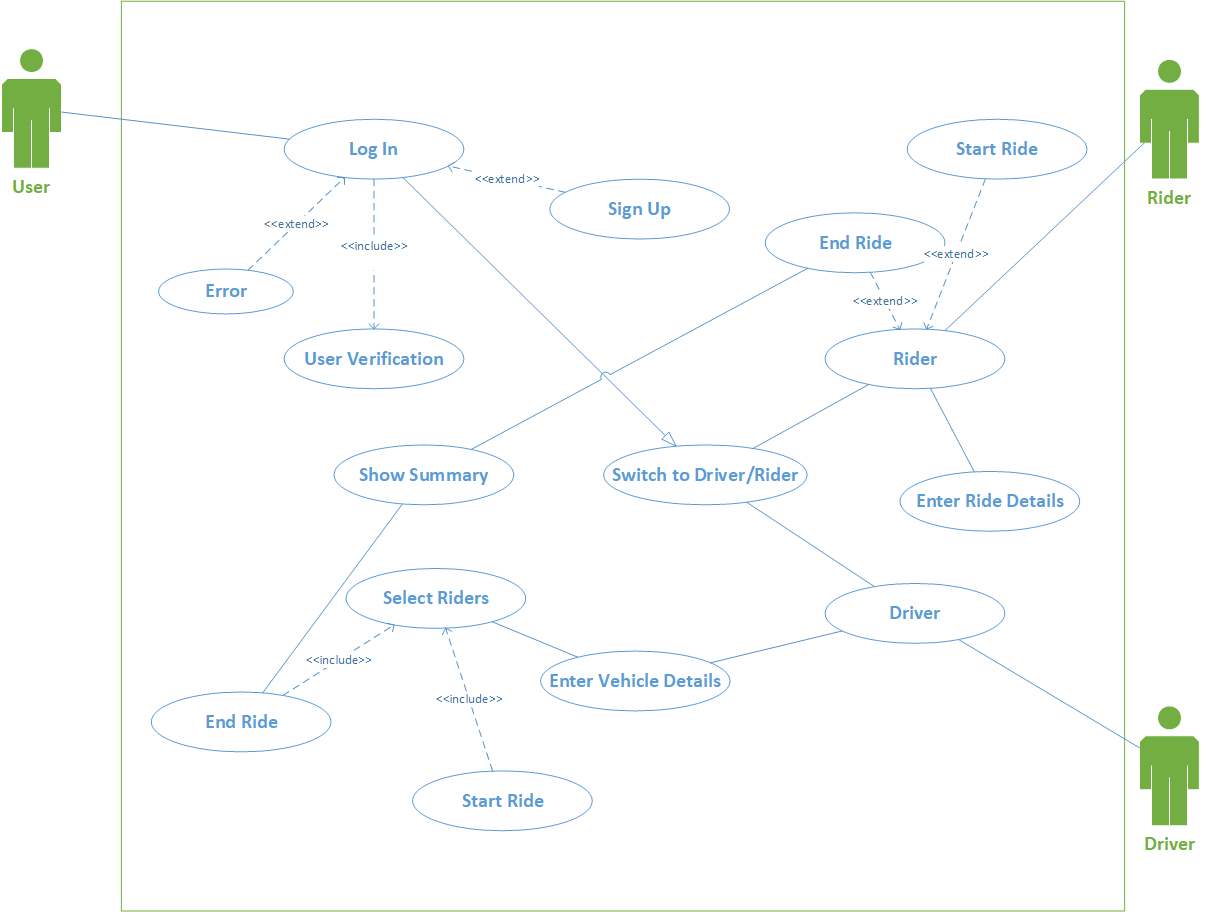
\includegraphics[width=1.0\textwidth]{UseCaseDiagram}
\caption{Use Case Diagram}
\label{fig:UseCaseDiagram}
\end{figure}

\begin{figure}[ht]
\subsection{Use Case Description}
\subsubsection{Table 17: Use Case - 01}
\centering
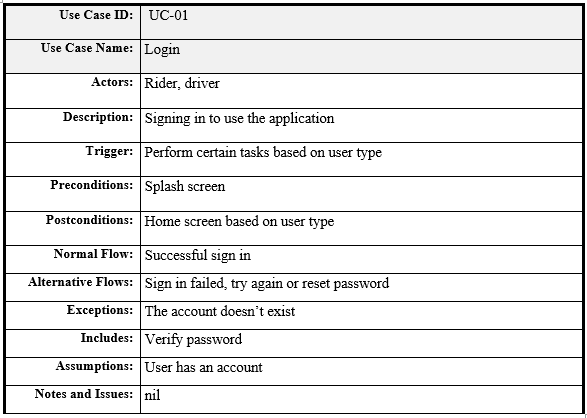
\includegraphics[width=0.8\textwidth]{TableUC1}
\end{figure}
\begin{figure}[ht]
\subsubsection{Table 18: Use Case - 02}
\centering
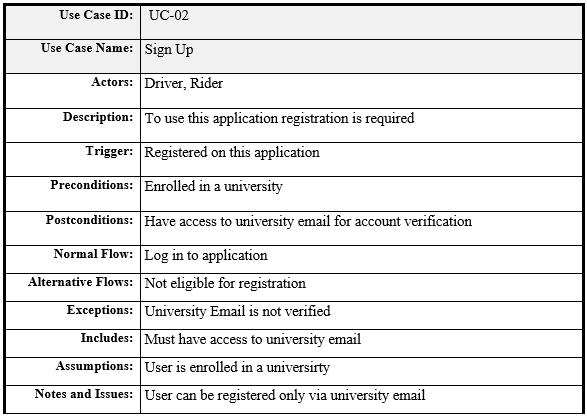
\includegraphics[width=0.8\textwidth]{TableUC2}
\end{figure}

\begin{figure}[ht]
\subsubsection{Table 19: Use Case - 03}
\centering
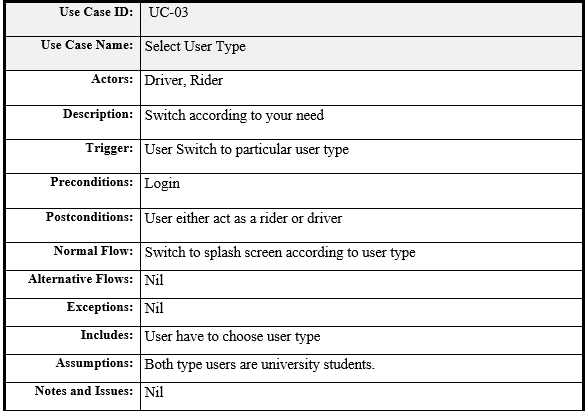
\includegraphics[width=0.8\textwidth]{TableUC3}
\end{figure}

\begin{figure}[ht]
\subsubsection{Table 20: Use Case - 04}
\centering
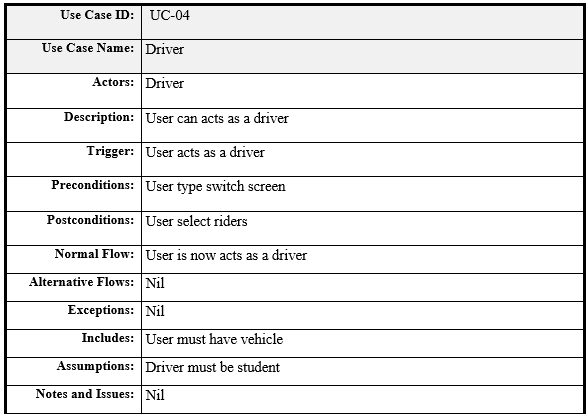
\includegraphics[width=0.8\textwidth]{TableUC4}
\end{figure}

\begin{figure}[ht]
\subsubsection{Table 21: Use Case - 05}
\centering
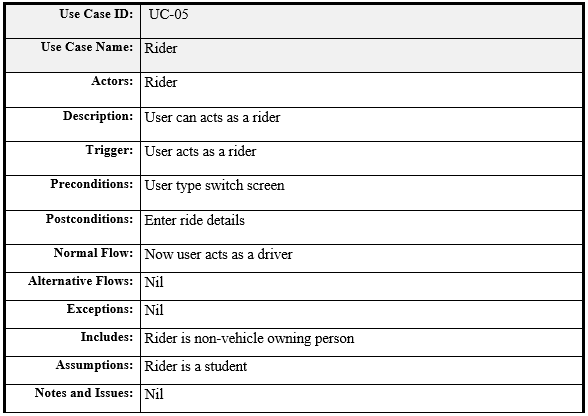
\includegraphics[width=0.8\textwidth]{TableUC5}
\end{figure}

\begin{figure}[ht]
\subsubsection{Table 22: Use Case - 06}
\centering
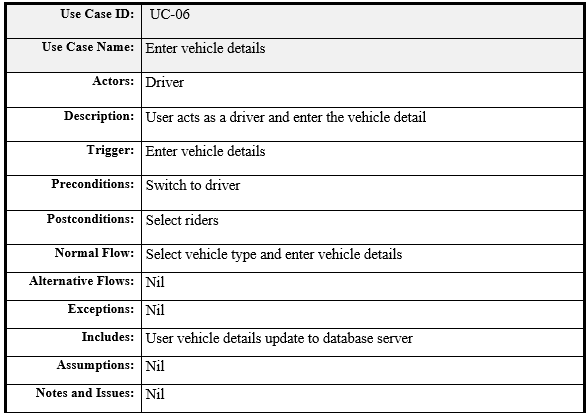
\includegraphics[width=0.8\textwidth]{TableUC6}
\end{figure}

\begin{figure}[ht]
\subsubsection{Table 23: Use Case - 07}
\centering
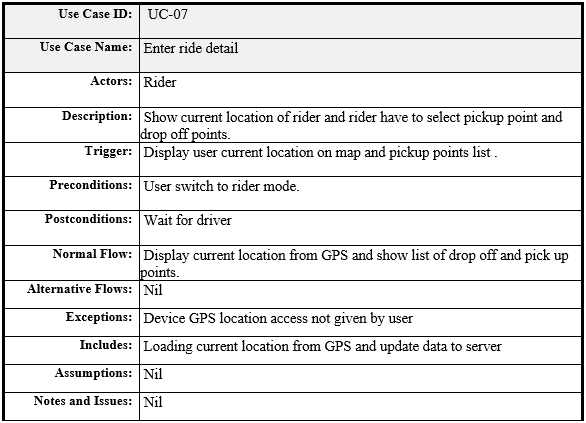
\includegraphics[width=0.8\textwidth]{TableUC7}
\end{figure}

\begin{figure}[ht]
\subsubsection{Table 24: Use Case - 08}
\centering
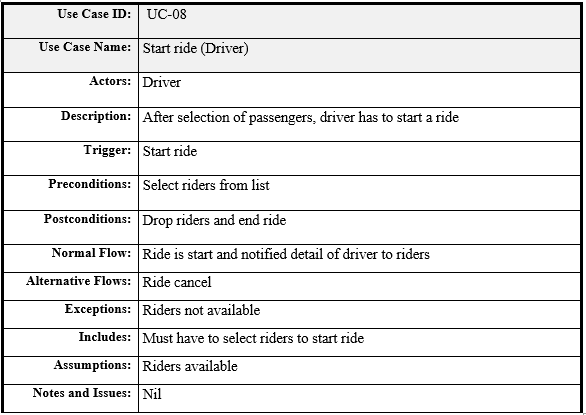
\includegraphics[width=0.8\textwidth]{TableUC8}
\end{figure}

\begin{figure}[ht]
\subsubsection{Table 25: Use Case - 09}
\centering
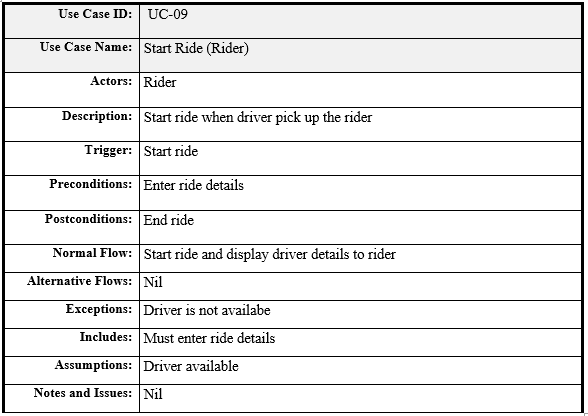
\includegraphics[width=0.8\textwidth]{TableUC9}
\end{figure}

\begin{figure}[ht]
\subsubsection{Table 26: Use Case - 10}
\centering
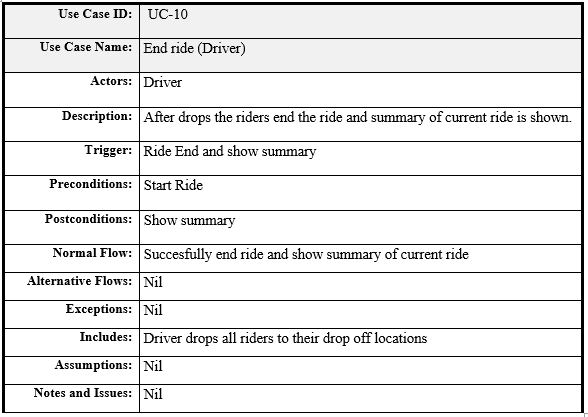
\includegraphics[width=0.8\textwidth]{TableUC10}
\end{figure}

\begin{figure}[ht]
\subsubsection{Table 27: Use Case - 11}
\centering
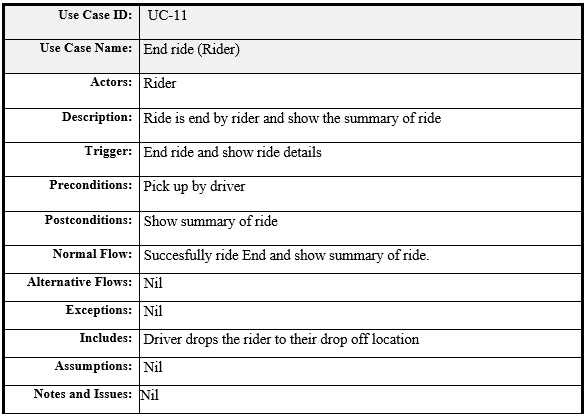
\includegraphics[width=0.8\textwidth]{TableUC11}
\end{figure}
 


\chapter{Design} \label{chap:design}

\section{System Architecture}
  
\subsection{High Level Context Diagram}
\begin{figure}[ht]
\center
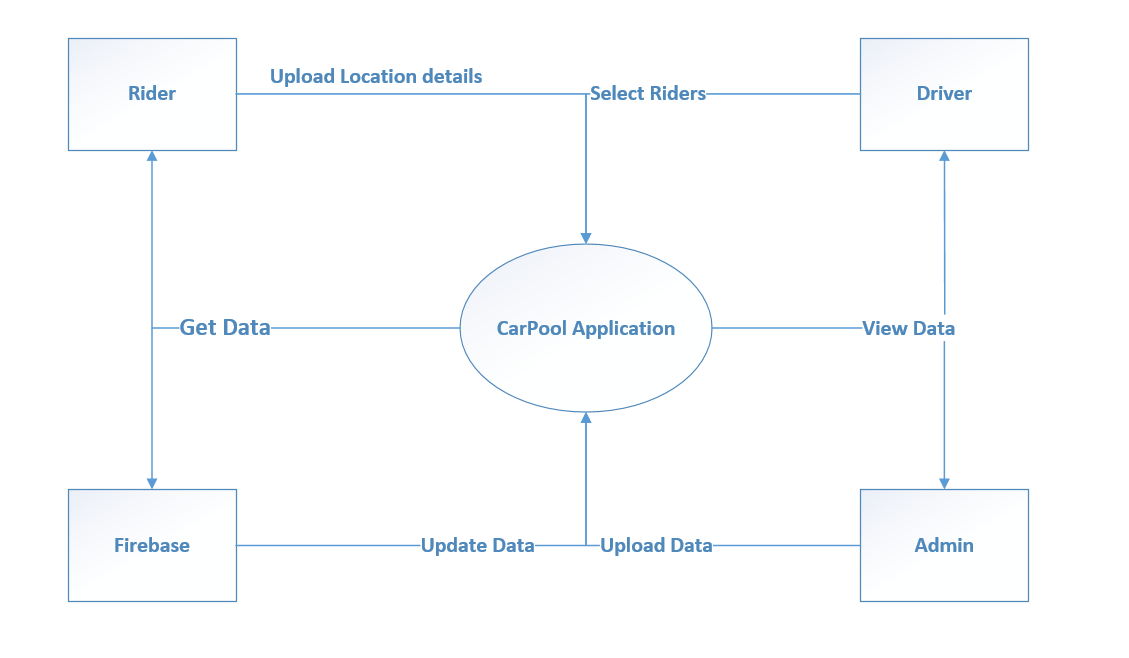
\includegraphics[width=1.2\textwidth]{SystemArchitecture}
\caption{Context Diagram}
\label{fig:Context Diagram}
\end{figure}
\begin{figure}[ht]
\center
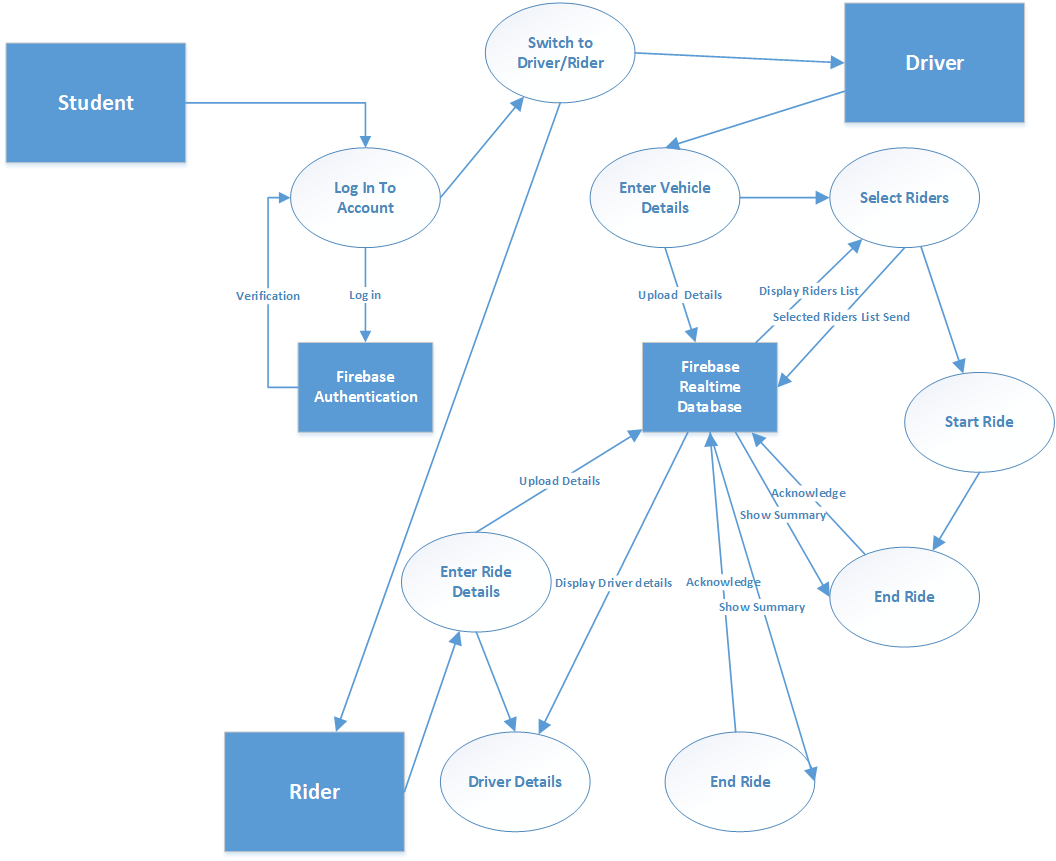
\includegraphics[width=1.0\textwidth]{SubSystem}
\caption{Sub System}
\label{fig:SubSystem}
\end{figure}

\section{Design Constraints} 
In our application we add a list of pick up points for the ease of drivers. This is made easier when clients can select pick up points and drivers reach the destination without hassle. Due to the COVID-19 pandemic, we could not be supervised and guided properly. Hence this process was not added and executed.

\section{Design Methodology}
The design of a project is important for the structure of the application by using UML (Unified Modeling Language) which is a general purpose modelling language, that aims to define a standard way to visualize the way a system has been designed. It is quite similar to blueprints used in other fields of engineering.
\\ \textbf{Reasons to use UML for project analysis and design are:} 

\begin{itemize}
\item Complex applications needs collaboration and planning, hence require a transparent and concise way to communicate amongst them.
\item A lot of time is saved down the road when team is able to visualize the processes, user interactions and static structure of the system. These project designs will try to make the general idea of the project more understandable and clearly understandable by identifying actors and functional / non-functional requirements, and also all the diagrams provide a transparent view about this project.
\end{itemize}



\begin{figure}
\section{High-Level Design}
\subsection{Conceptual or Logical: UML Package diagram} 
\center
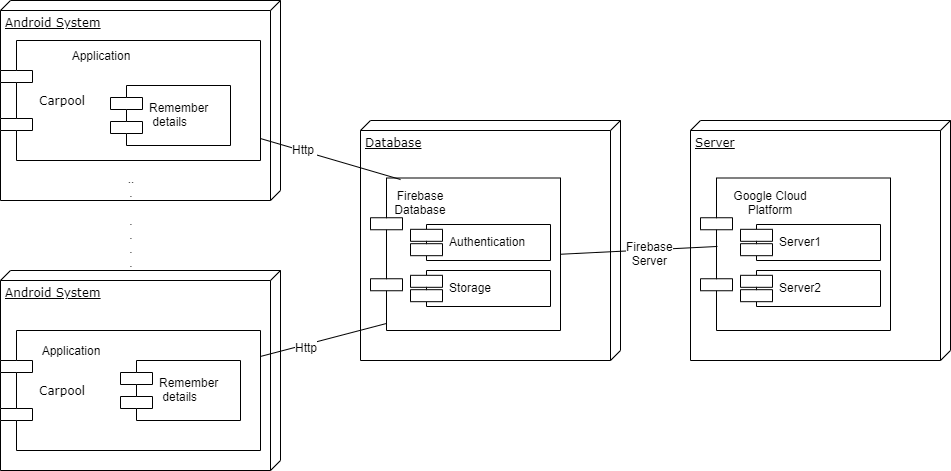
\includegraphics[width=1.0\textwidth]{PackageDiagram}
\caption{Package Diagram}
\label{fig:Package Diagram}
\end{figure}

\begin{figure}
\subsection{Process Interaction Diagram}
\center
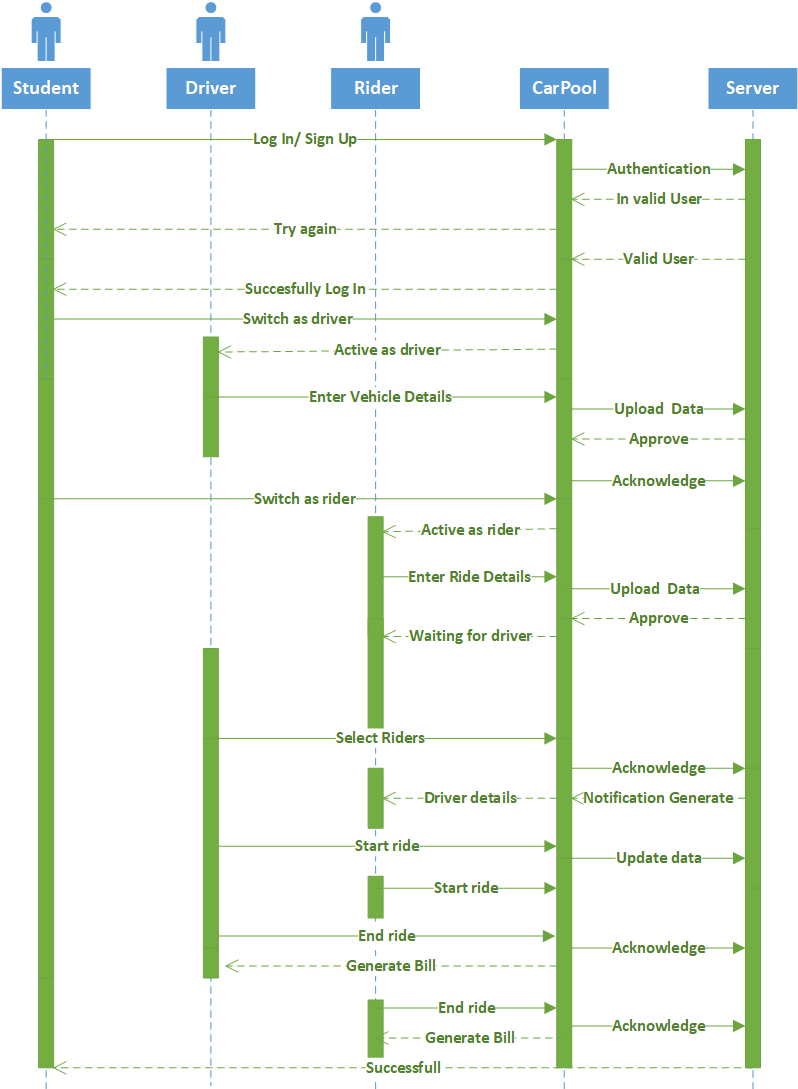
\includegraphics[width=15cm,height=25cm,keepaspectratio]{InteractionDiagram}
\caption{Process Interaction Diagram}
\label{fig:Process Interaction Diagram}
\end{figure}

\begin{figure}
\subsection{Physical Deployment Diagram}
\center
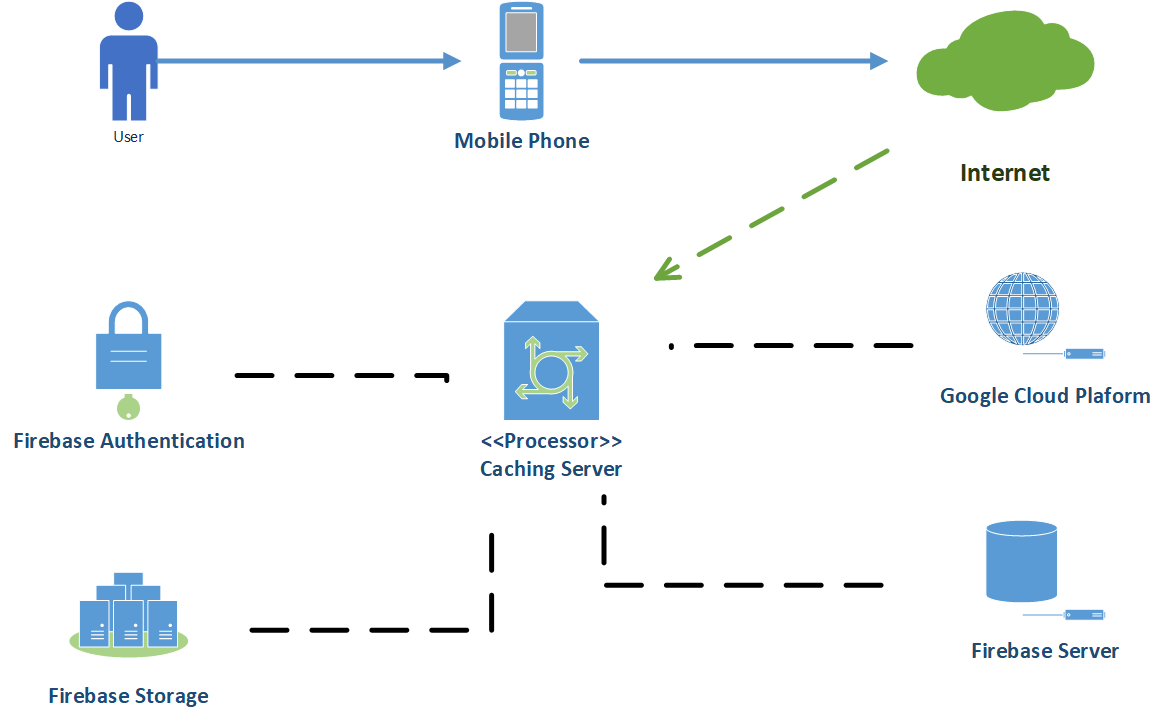
\includegraphics[width=15cm,height=20cm,keepaspectratio]{DeploymentDiagram}
\caption{Deployment Diagram}
\label{fig:Deployment Diagram}
\end{figure}

\begin{figure}
\subsection{Modules}
The application is divided into three modules
\begin{itemize}
\item User Registration
\item Driver
\item Rider
\end{itemize}
\end{figure}

\begin{figure}
\subsubsection{User Registration}
In this module, the user must register their credentials to use this application. Users should be student and currently enrolled in Air University. The user should enter the details first name, last Name, student email, university registration id, contact no, password. So user using these registration details will be able to use application. This authentication process to avoid someone malpractice as this application is verifying student details.
\end{figure}

\begin{figure}
\subsubsection{Driver}
In this module, the user acts as a driver. This module is consist of 8 activities which contains 2 fragments (map, passenger list), the driver can use the map fragment to see the passenger pickup points and current location and passenger list fragment to see the list of passengers. Driver module also contains the activities of enter vehicle details, summary of ride.
\end{figure}

\begin{figure}
\subsubsection{Rider}
In this module, the user acts as a rider. This module is consist of 4 activities  which contains 2 fragments (map, driver details), the passenger can use the map fragment to see the pickup point and current location and driver detail fragment to see the detail of driver. Rider module also contains the activities to enter trip detail, summary of ride.
\end{figure}

\begin{figure}
\subsection{Security} 		
This application should never disclose any personal information of any user, and should collect no personal information from it's own users.
\end{figure}

\begin{figure}
\section{Low Level Design} 
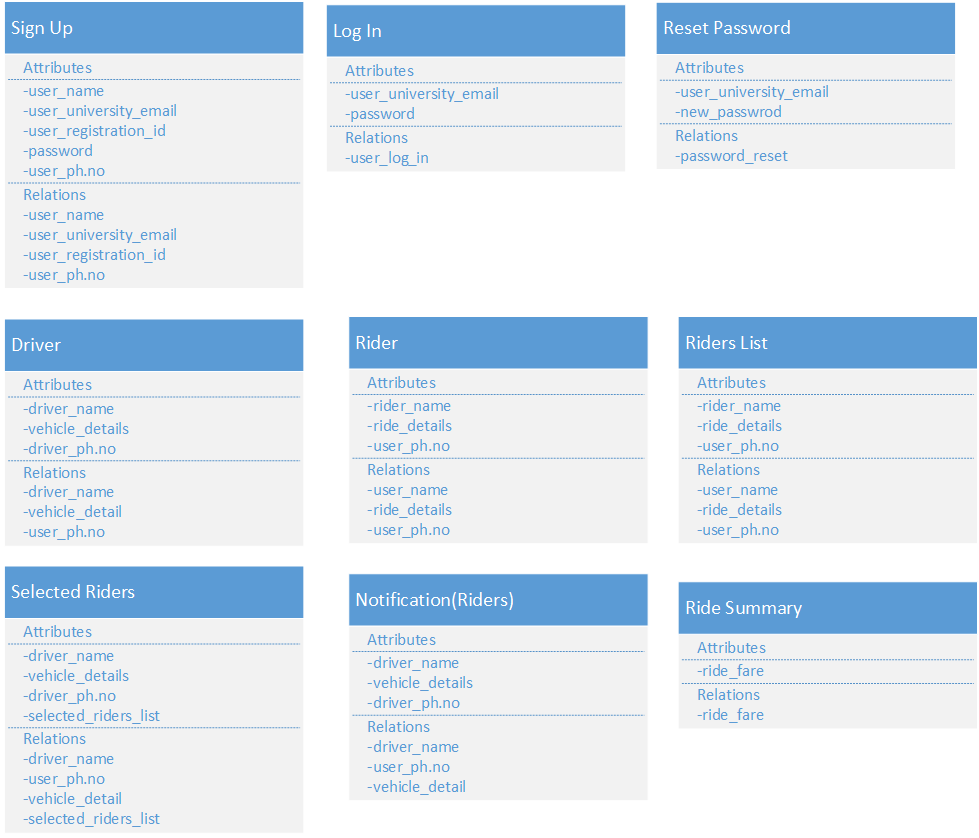
\includegraphics[width=16cm,height=25cm,keepaspectratio]{LowLevelDesign}
\caption{Low Level Design}
\label{fig:Low Level Design}
\center
\end{figure}

\begin{figure}
\section{Database Design}
Firebase platform provides a cloud-hosted real time database. It is a NoSQL cloud database. Data synchronizes among all clients and stays available even when the app goes offline. As it is a NoSQL database, so its functionality is different as compared to a relational database. The data is stored in the form of collections and documents. There is no relationship between classes, so there won’t be any schema of our database. Data gets stored as JSON Objects. it is more like a cloud-hosted JSON tree. When a person adds data to the JSON tree, it becomes a node in the existing JSON structure with an associated key. The best method is to use the denormalization technique; using which we split data into separate paths. It becomes easier to download the data in separate calls as required.
\end{figure}

\begin{figure}
\section{GUI Design}
Our application contains more than fifteen screens, different screens based on user type are:
\end{figure}

\begin{figure}
\subsection{Welcome Interface}
This is the interface that shows up to the user when he’s open the application, this interface is composed of the application’s name, a logo and a slang which describe the application alongside an “Get Started” button which lets the user to log in screen.
\begin{center}
\subfloat[Welcome Screen]{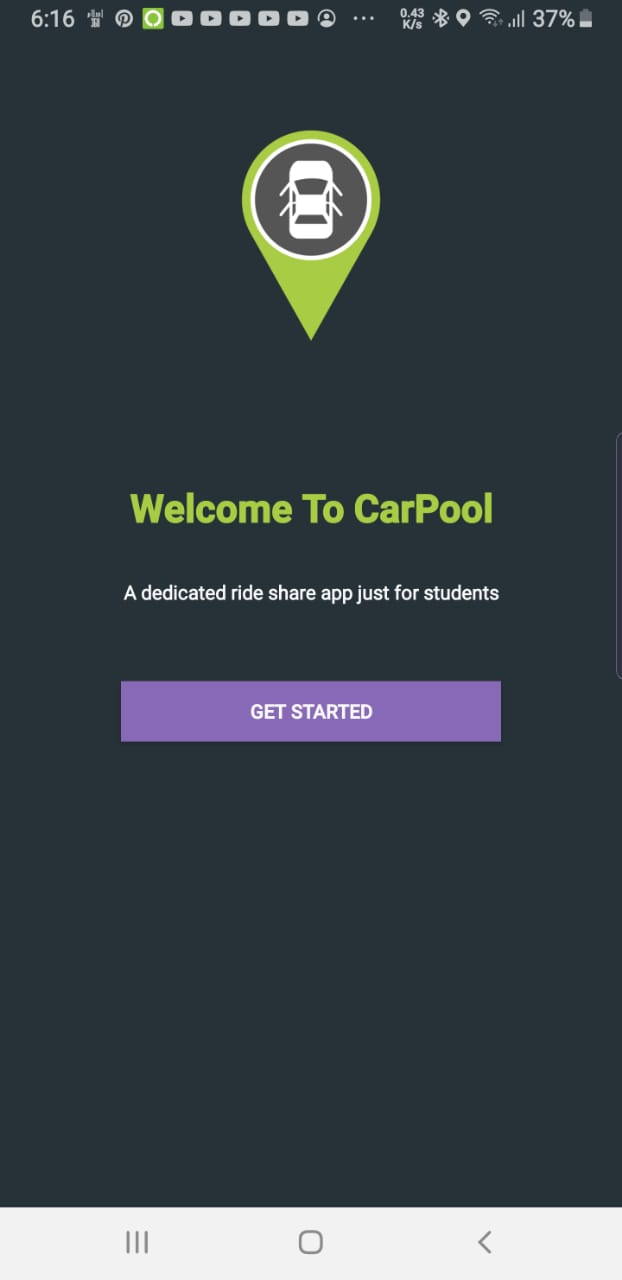
\includegraphics[width = 2in]{S1}}
\end{center}
\subsection{Authentication Interfaces}
The authentication interface is made as simple as possible while also being very beautiful and professional, it utilizes Firebase auth as a backend which allows for a secure connection to the database plus encrypted passwords for extra security, this interface also contains options to recover password in case the user has forgotten their password.

\end{figure}

\begin{figure}
\hspace*{\fill}
\subfloat[Login Screen]{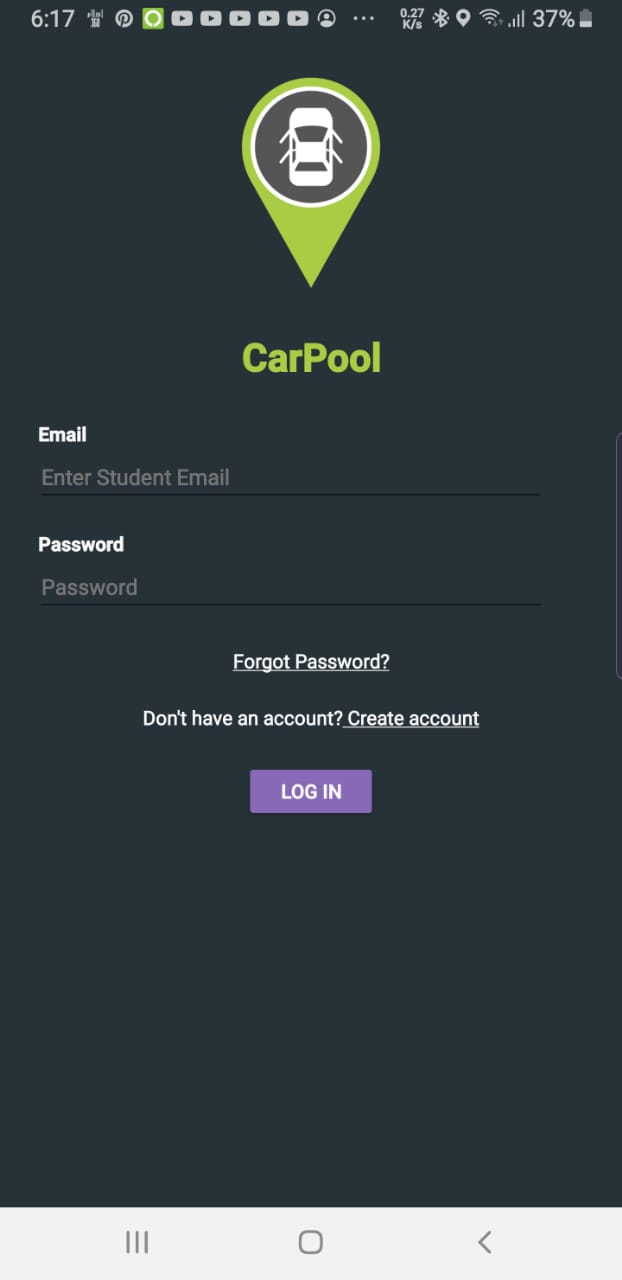
\includegraphics[width = 2in]{S2}}\hfill 
\subfloat[Signup Screen]{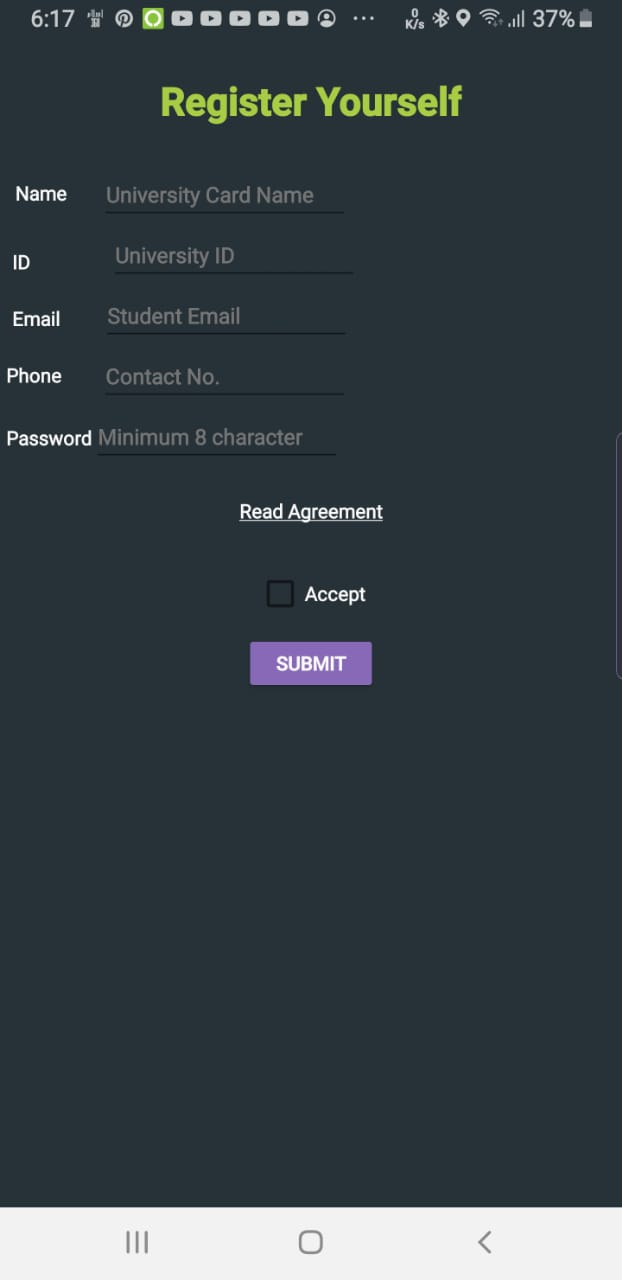
\includegraphics[width = 2in]{S3}}
\hspace*{\fill}
\end{figure}

\begin{figure}
\centering
\subfloat[Forgot Password Screen]{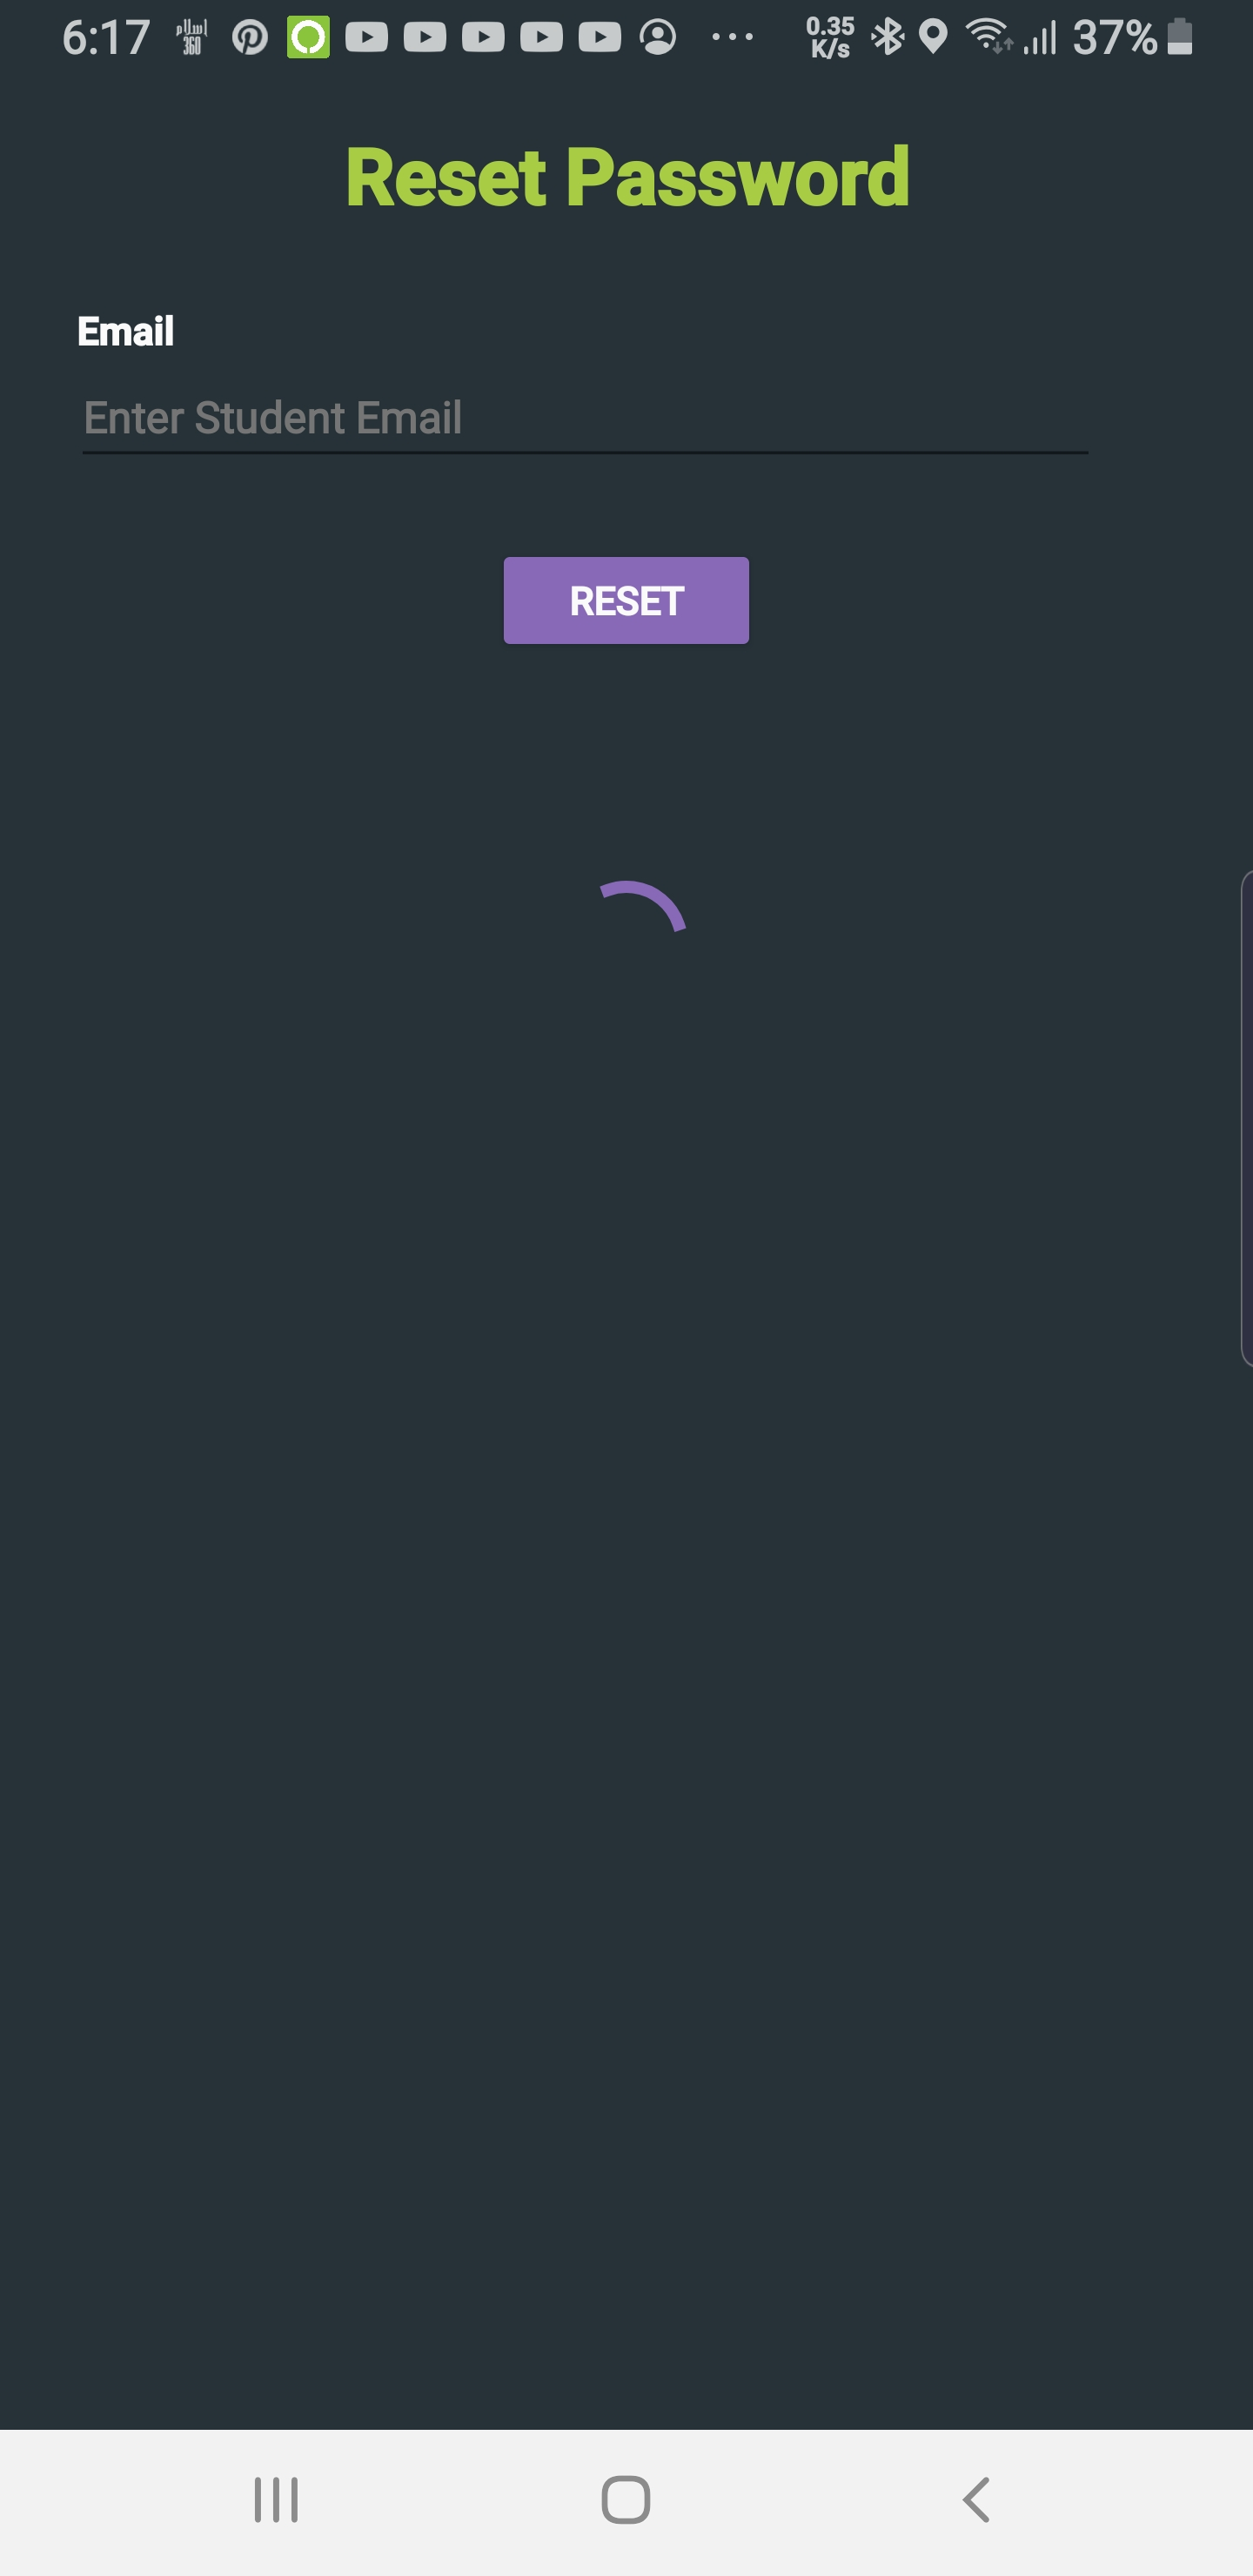
\includegraphics[width = 2in]{S4}}
\end{figure}

\begin{figure}
\subsection{Type Switching Interface}
This is the interface that shows up to the user when he’s logged in into the application, this interface is composed of the application’s name and a logo alongside a switch button, which lets the user to their selected user type interface.
\begin{center}
\subfloat[Select User Type Screen]{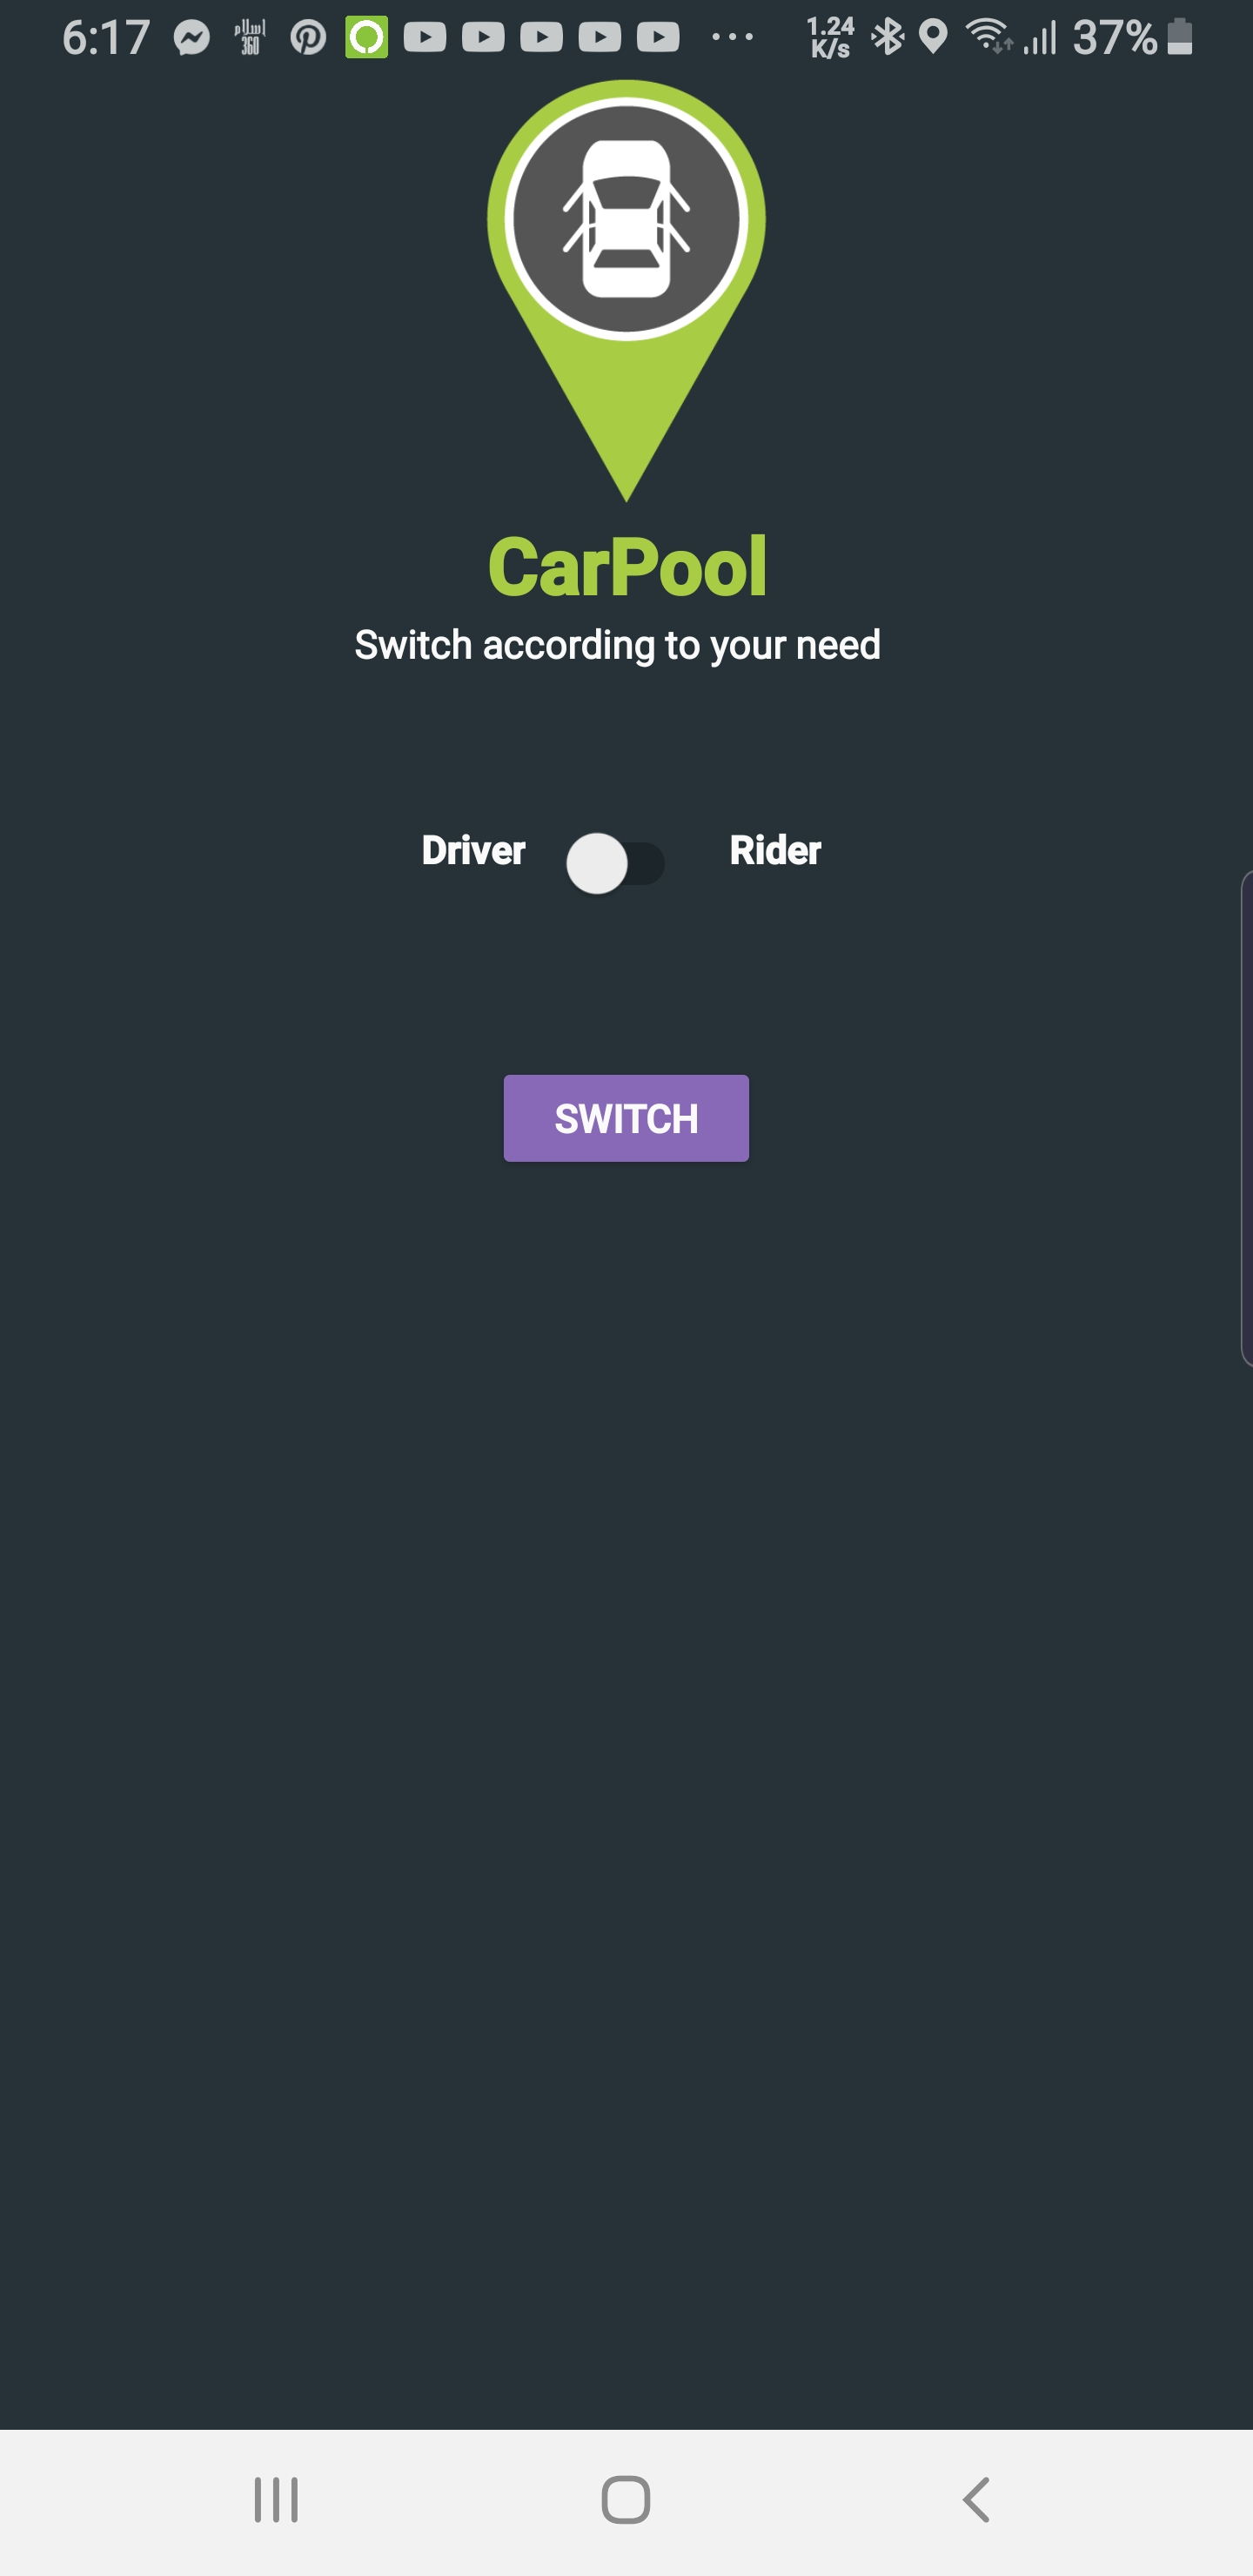
\includegraphics[width = 2in]{S5}}
\end{center}
\subsection{Rider Interfaces}
These interfaces are used by the passengers to post a ride details for drivers to see and select riders, these interfaces is extremely customizable and professional, by using Google Places API, Google Direction API, Google Map API in these interfaces. We have created a very organized and efficient algorithm to optimize the results when Passengers search for a driver, when rider picks an origin and a destination using Places AutoComplete API, the algorithm uses a combination of Geolocation and Places API to find the full address, city and sub city, then it converts the city into a number and saves all the information in the trip object for it to be saved into the database later.
\end{figure}

\begin{figure} 
\hspace*{\fill}
\subfloat[Enter Ride Detail Screen]{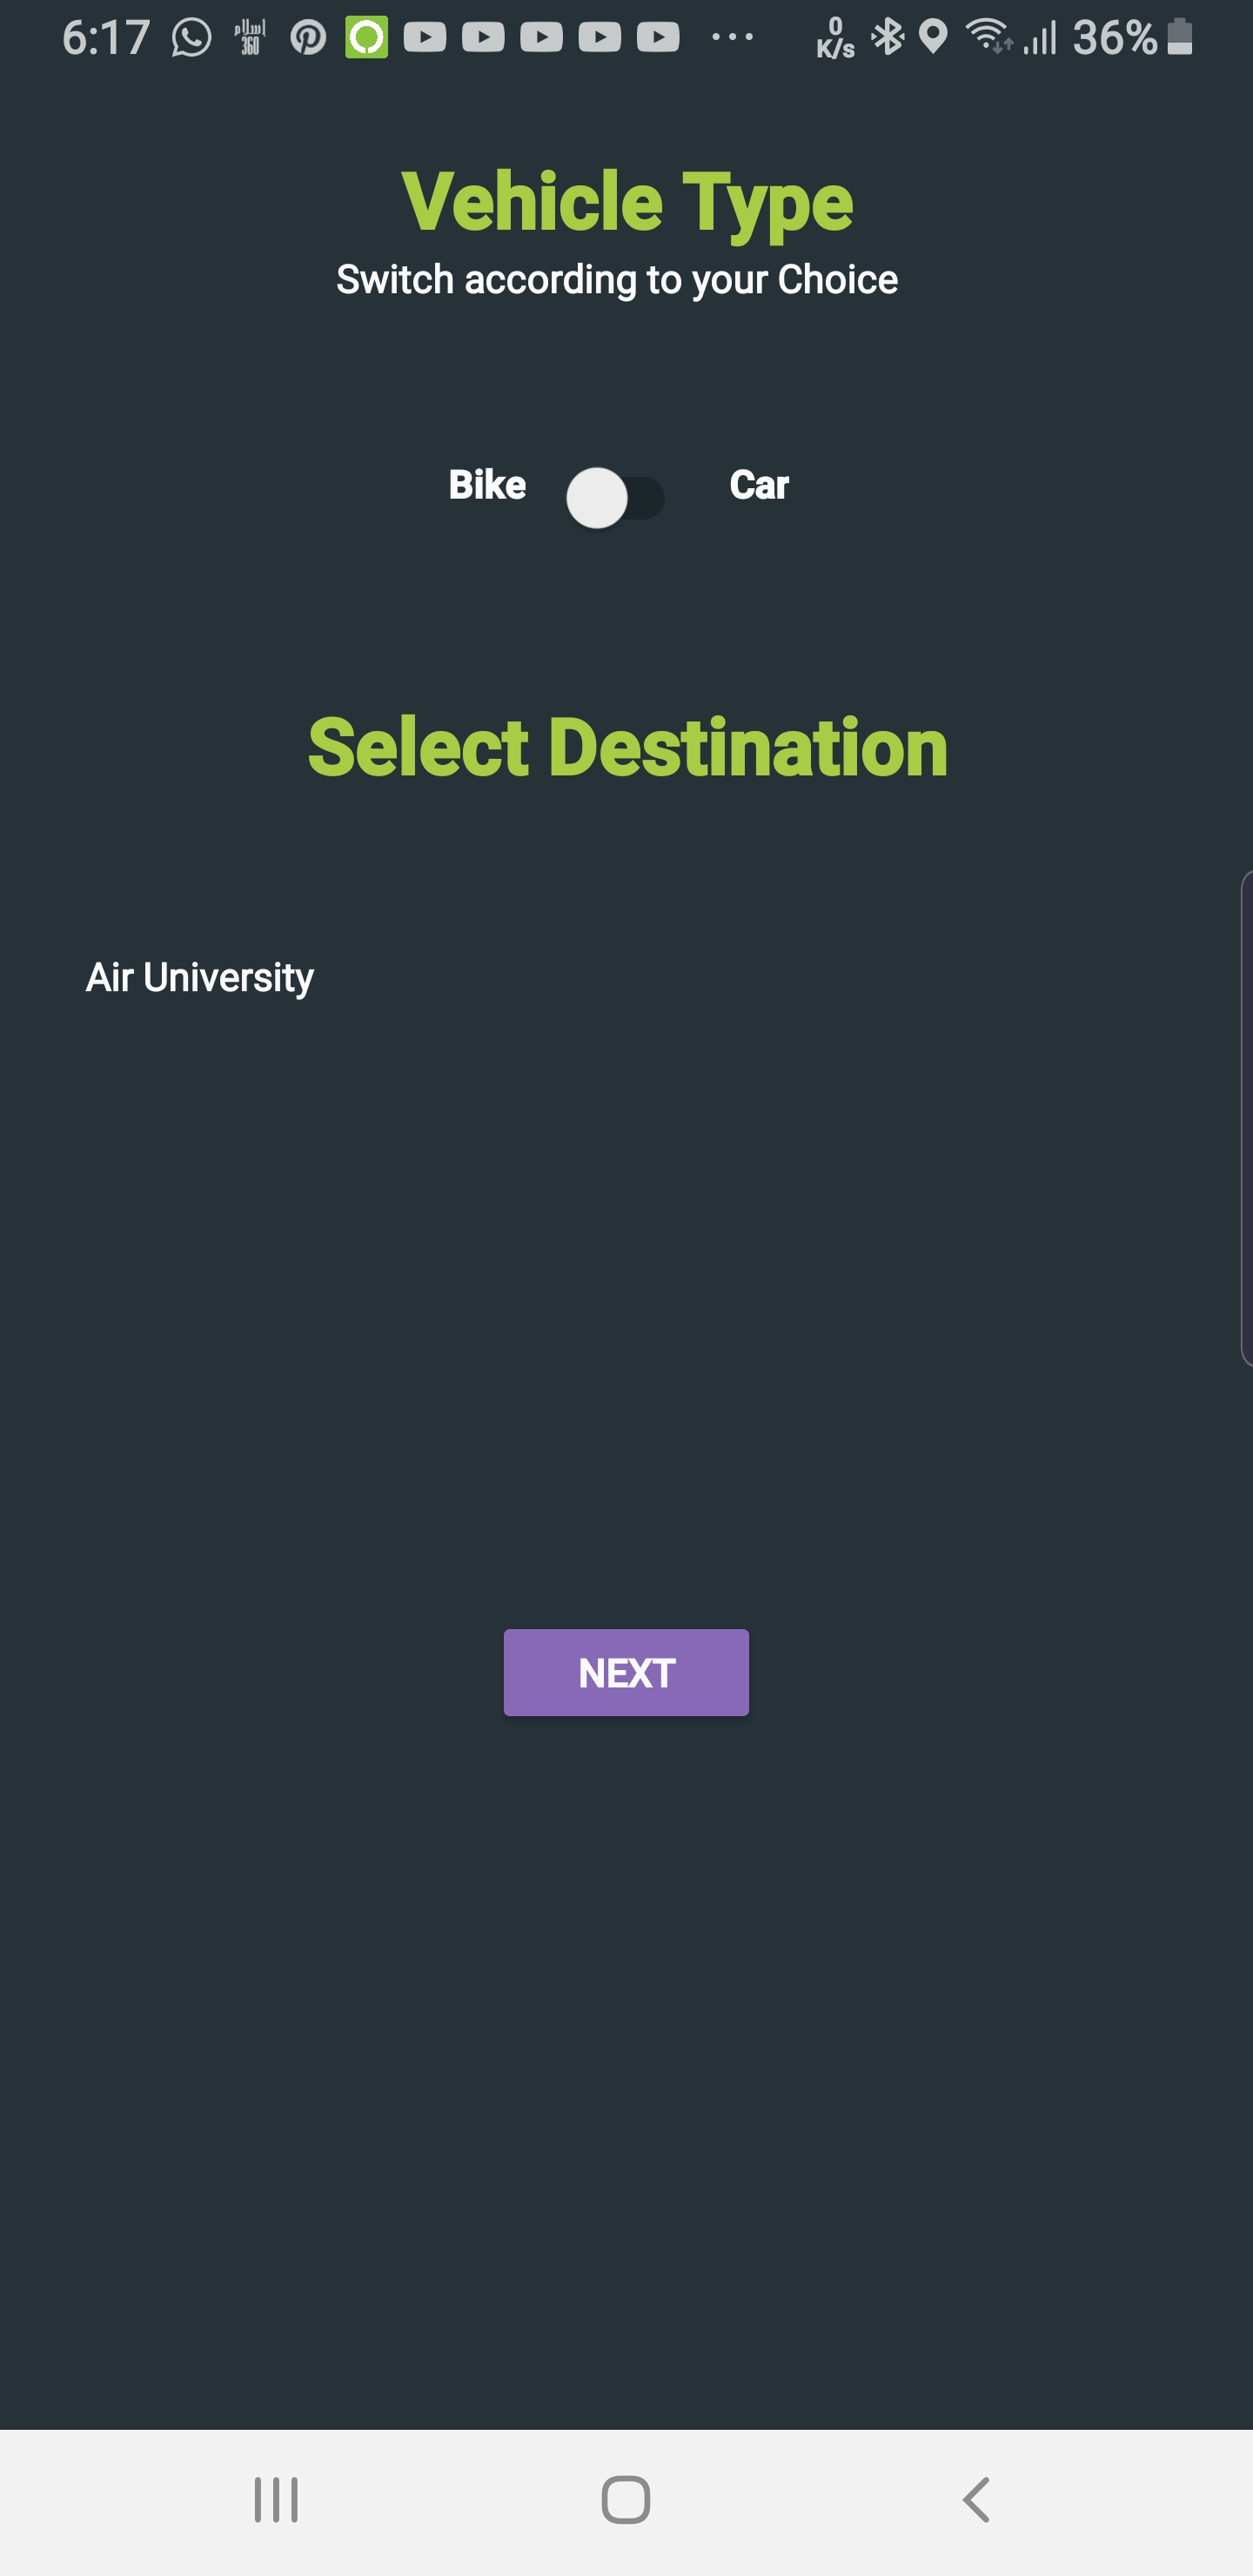
\includegraphics[width = 2in]{S6}}\hfill 
\subfloat[Map Screen]{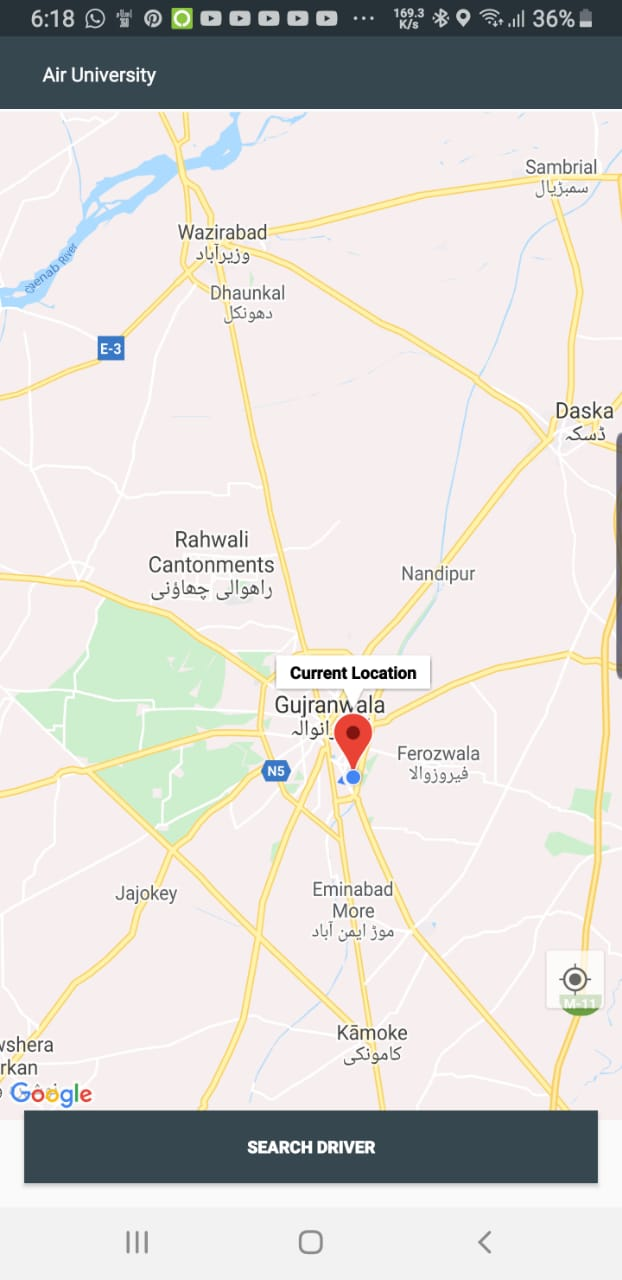
\includegraphics[width = 2in]{S7}}
\hspace*{\fill}
\end{figure}

\begin{figure}
\hspace*{\fill}
\subfloat[Driver Detail Screen]{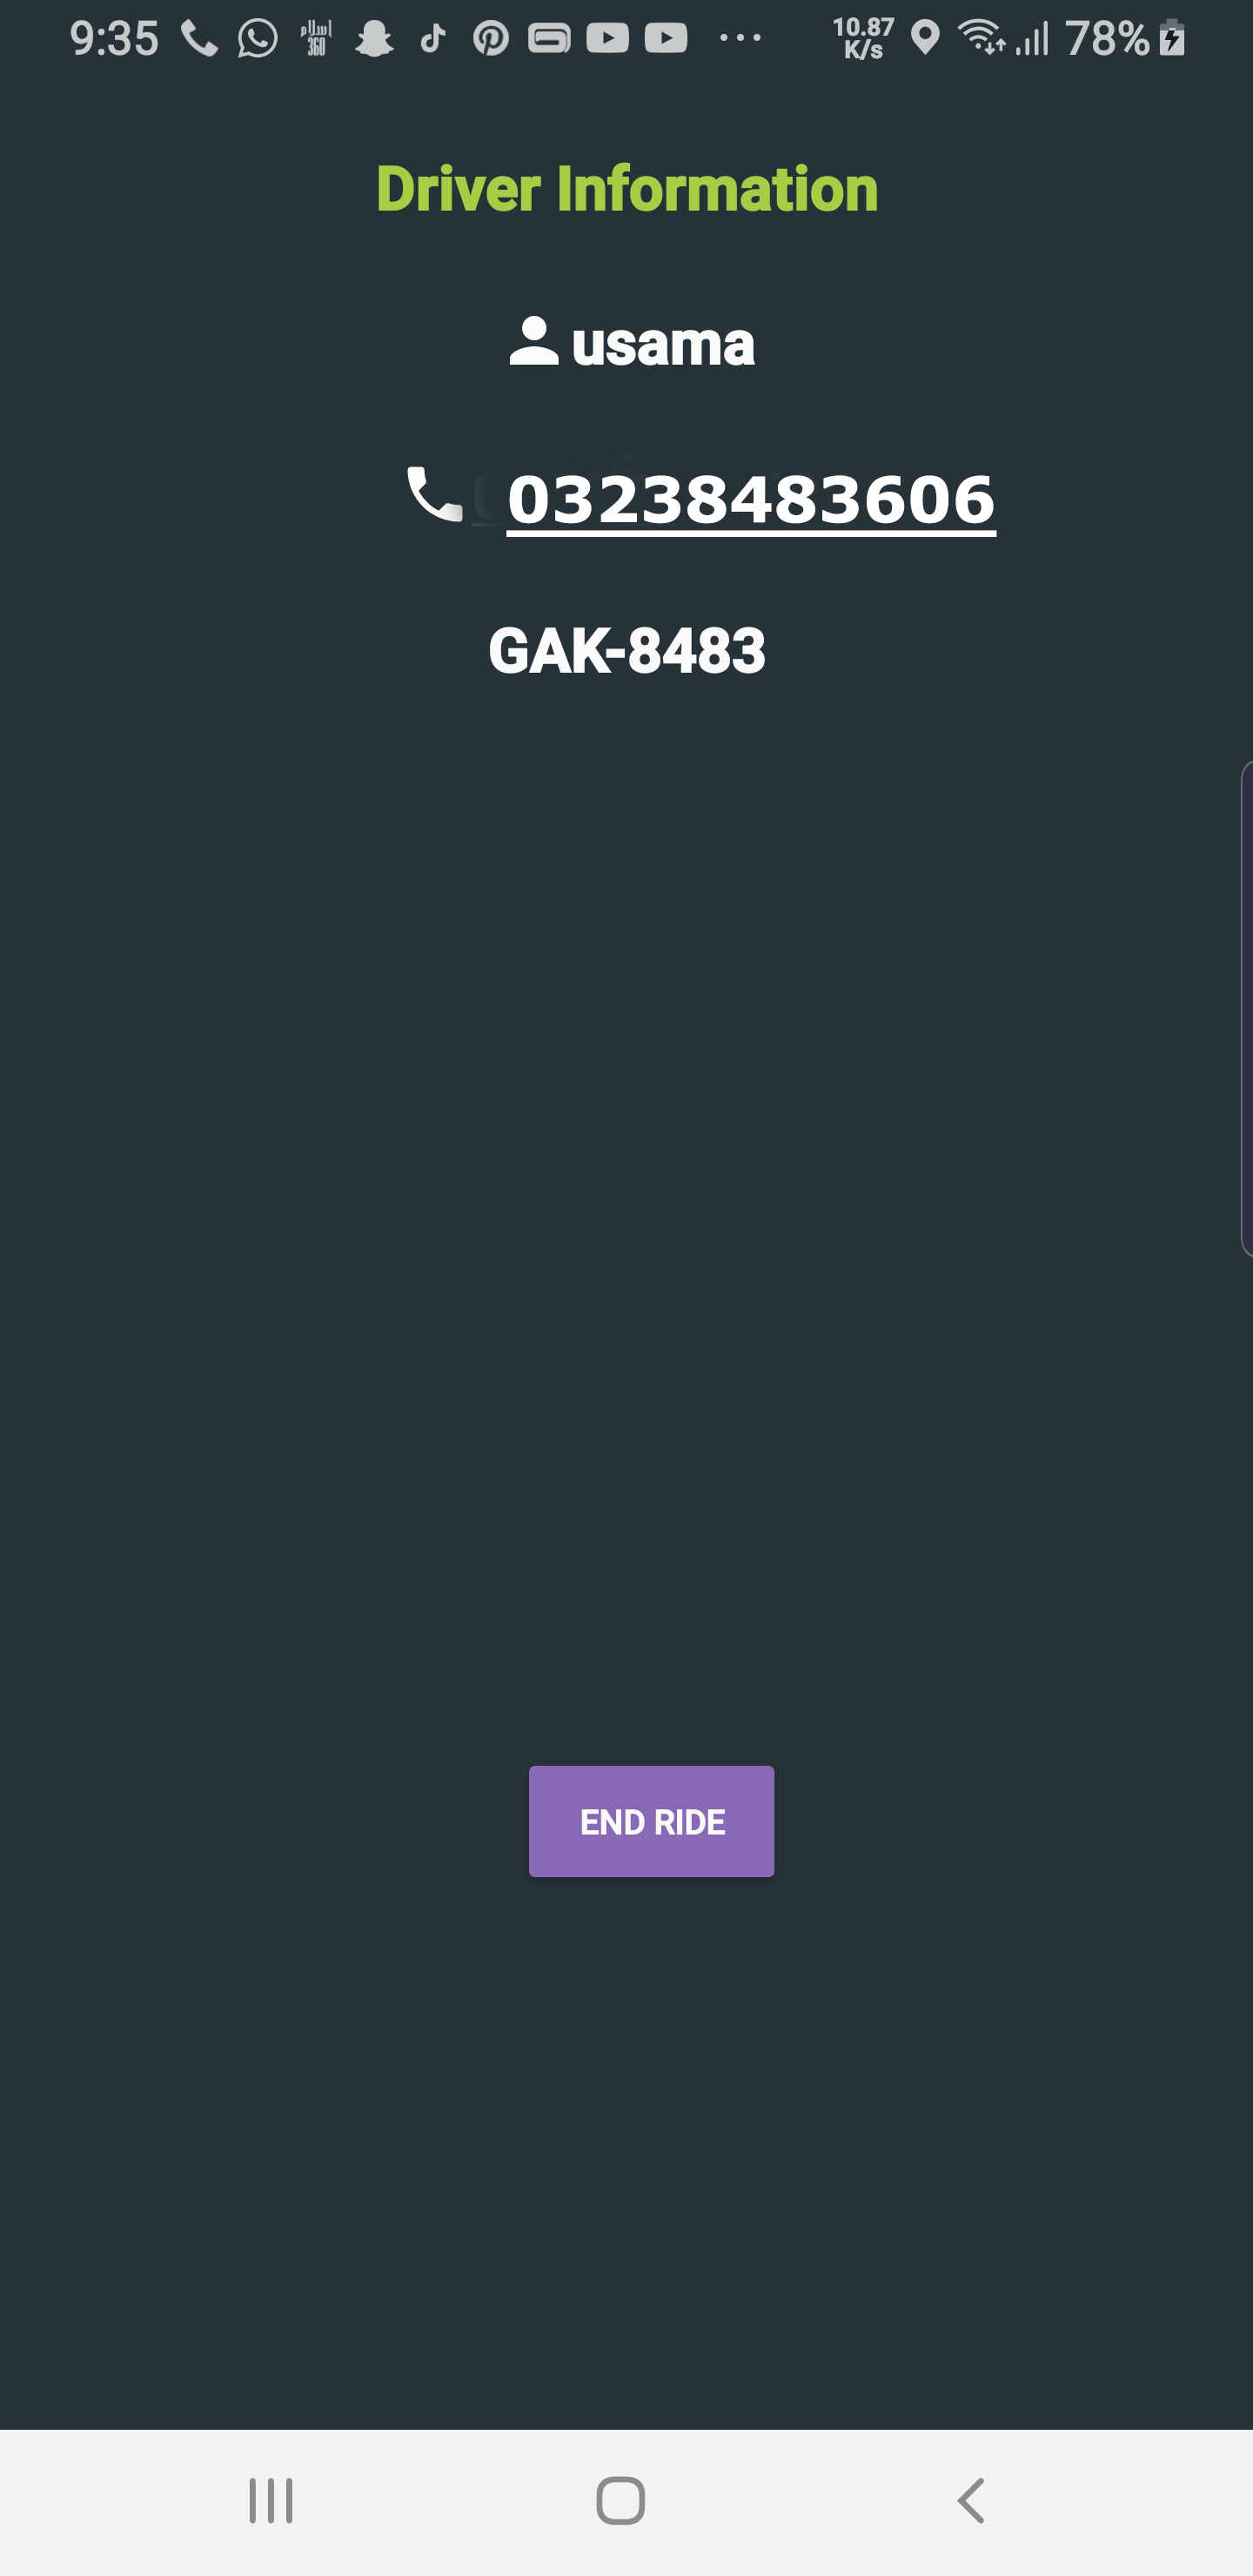
\includegraphics[width = 2in]{S8}}\hfill 
\subfloat[Ride Summary Screen]{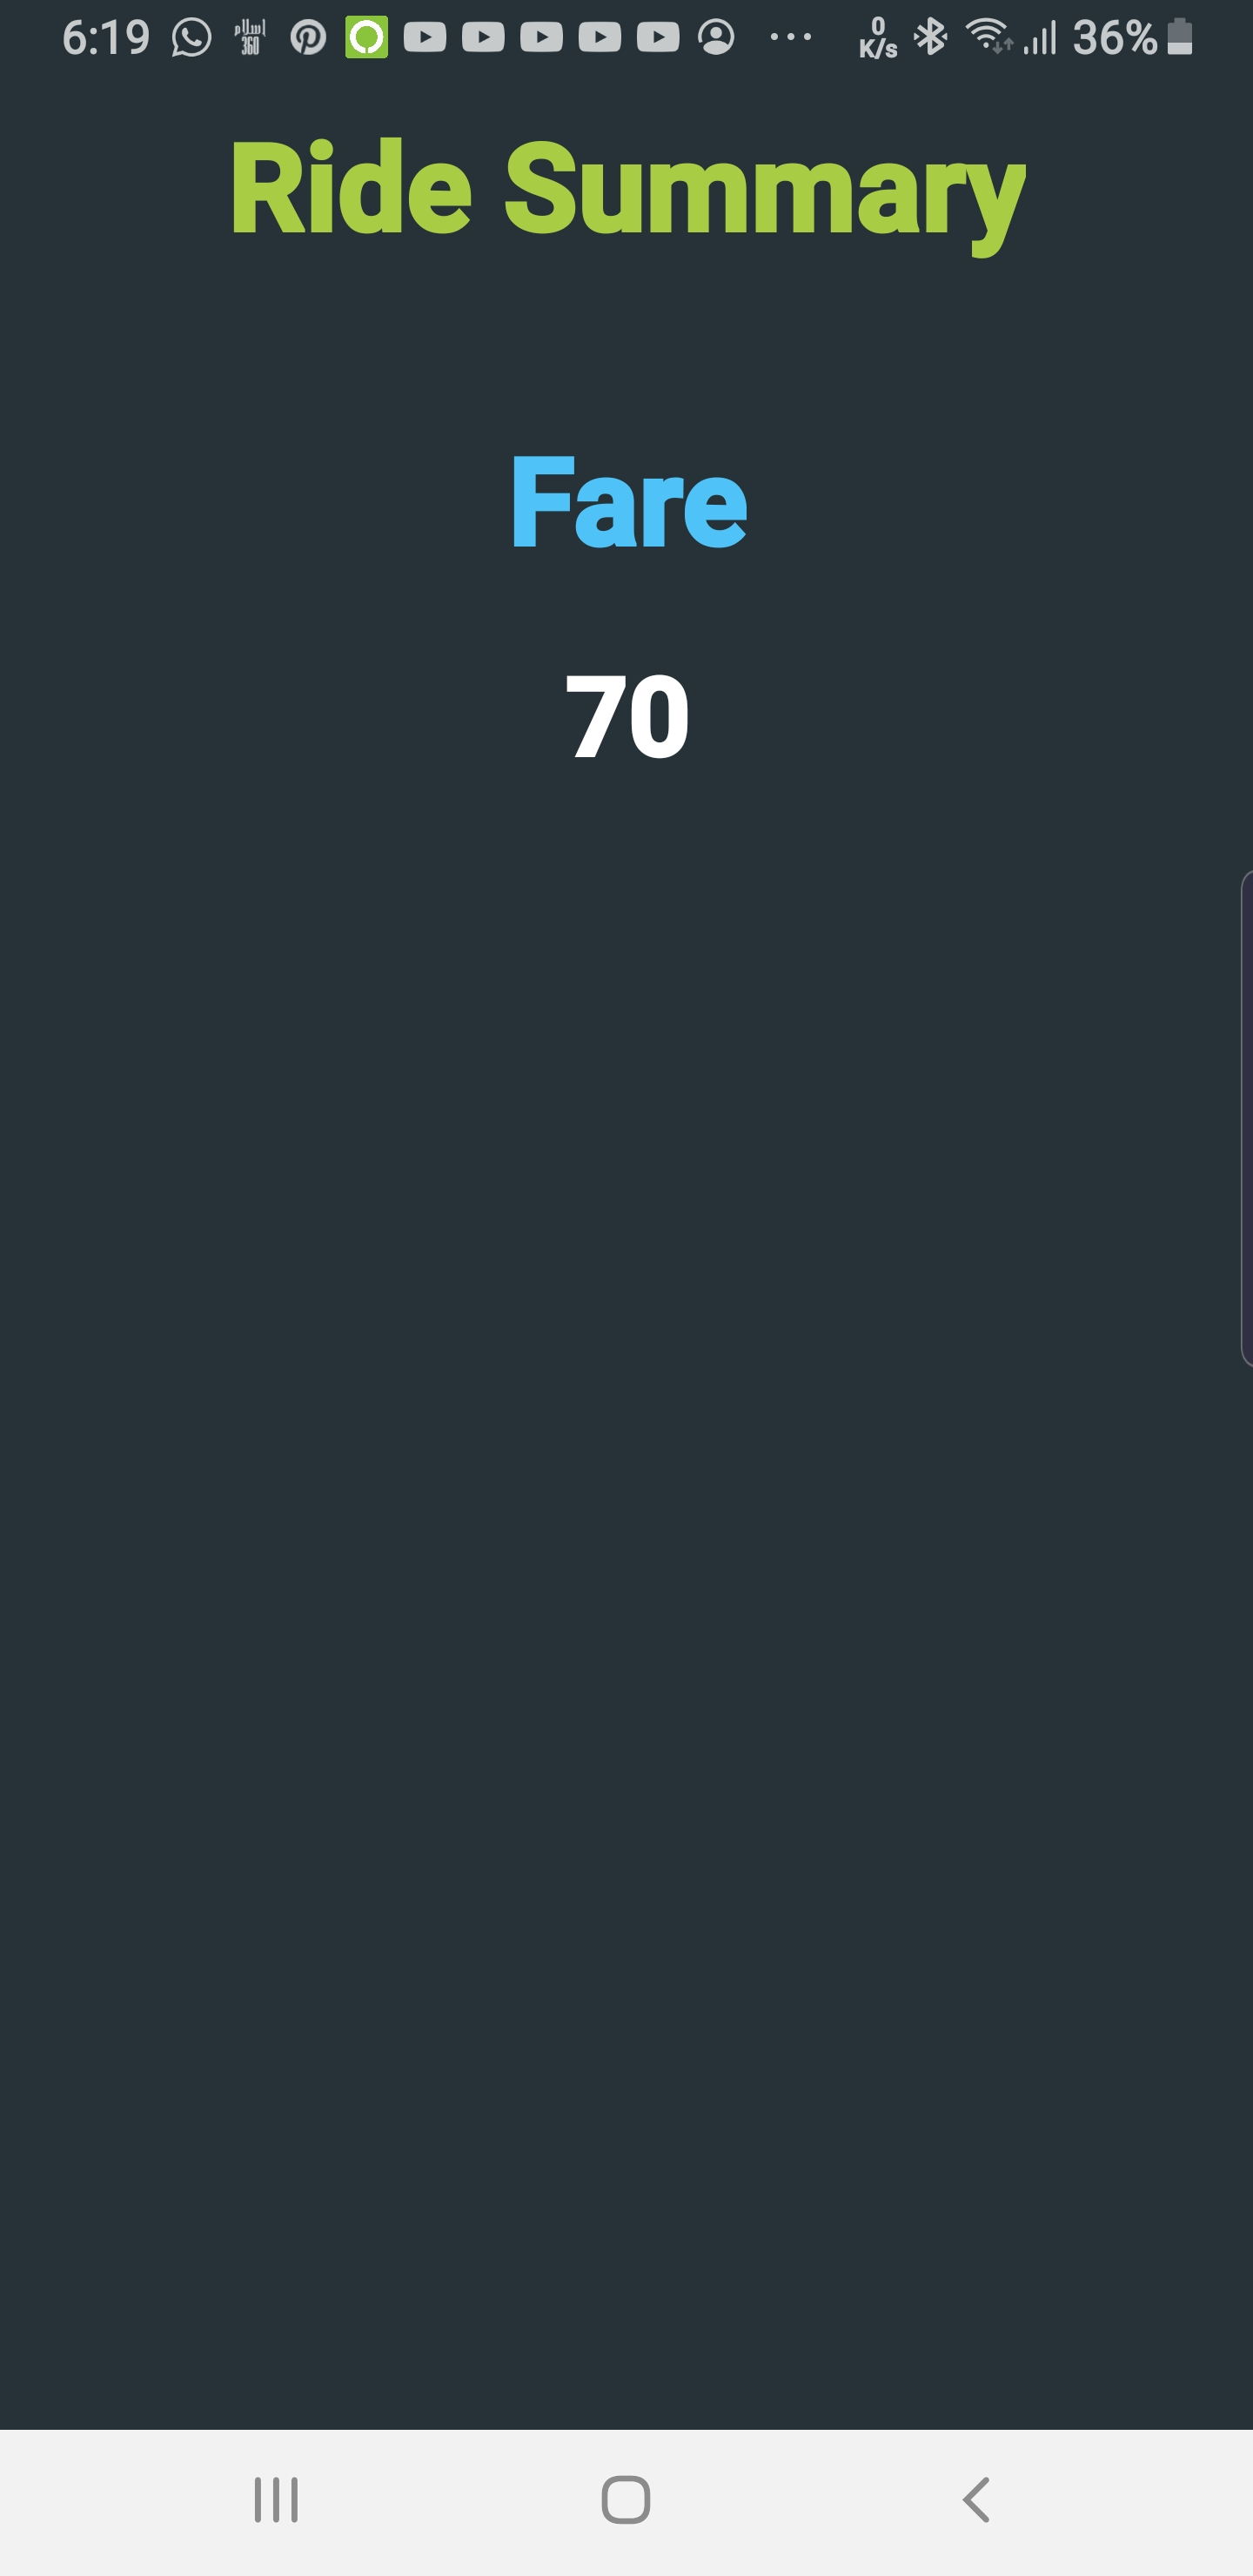
\includegraphics[width = 2in]{S9}}
\hspace*{\fill}
\end{figure}

\begin{figure}
\subsection{Driver Interfaces}
These interfaces are used by rider to enter vehicle detail, see and select the passengers for trip, these form is extremely customizable and professional, by using Google Places API in this interface we have created a very organized and efficient algorithm to optimize the results, when the driver select riders using Places AutoComplete API, the algorithm uses a combination of Geolocation and Places API to find the full address, city and sub city, then it converts the city into a number and saves all the information in the trip object for it to be saved into the database later.
\hspace*{\fill}
\subfloat[Enter Vehicle Detail Screen]{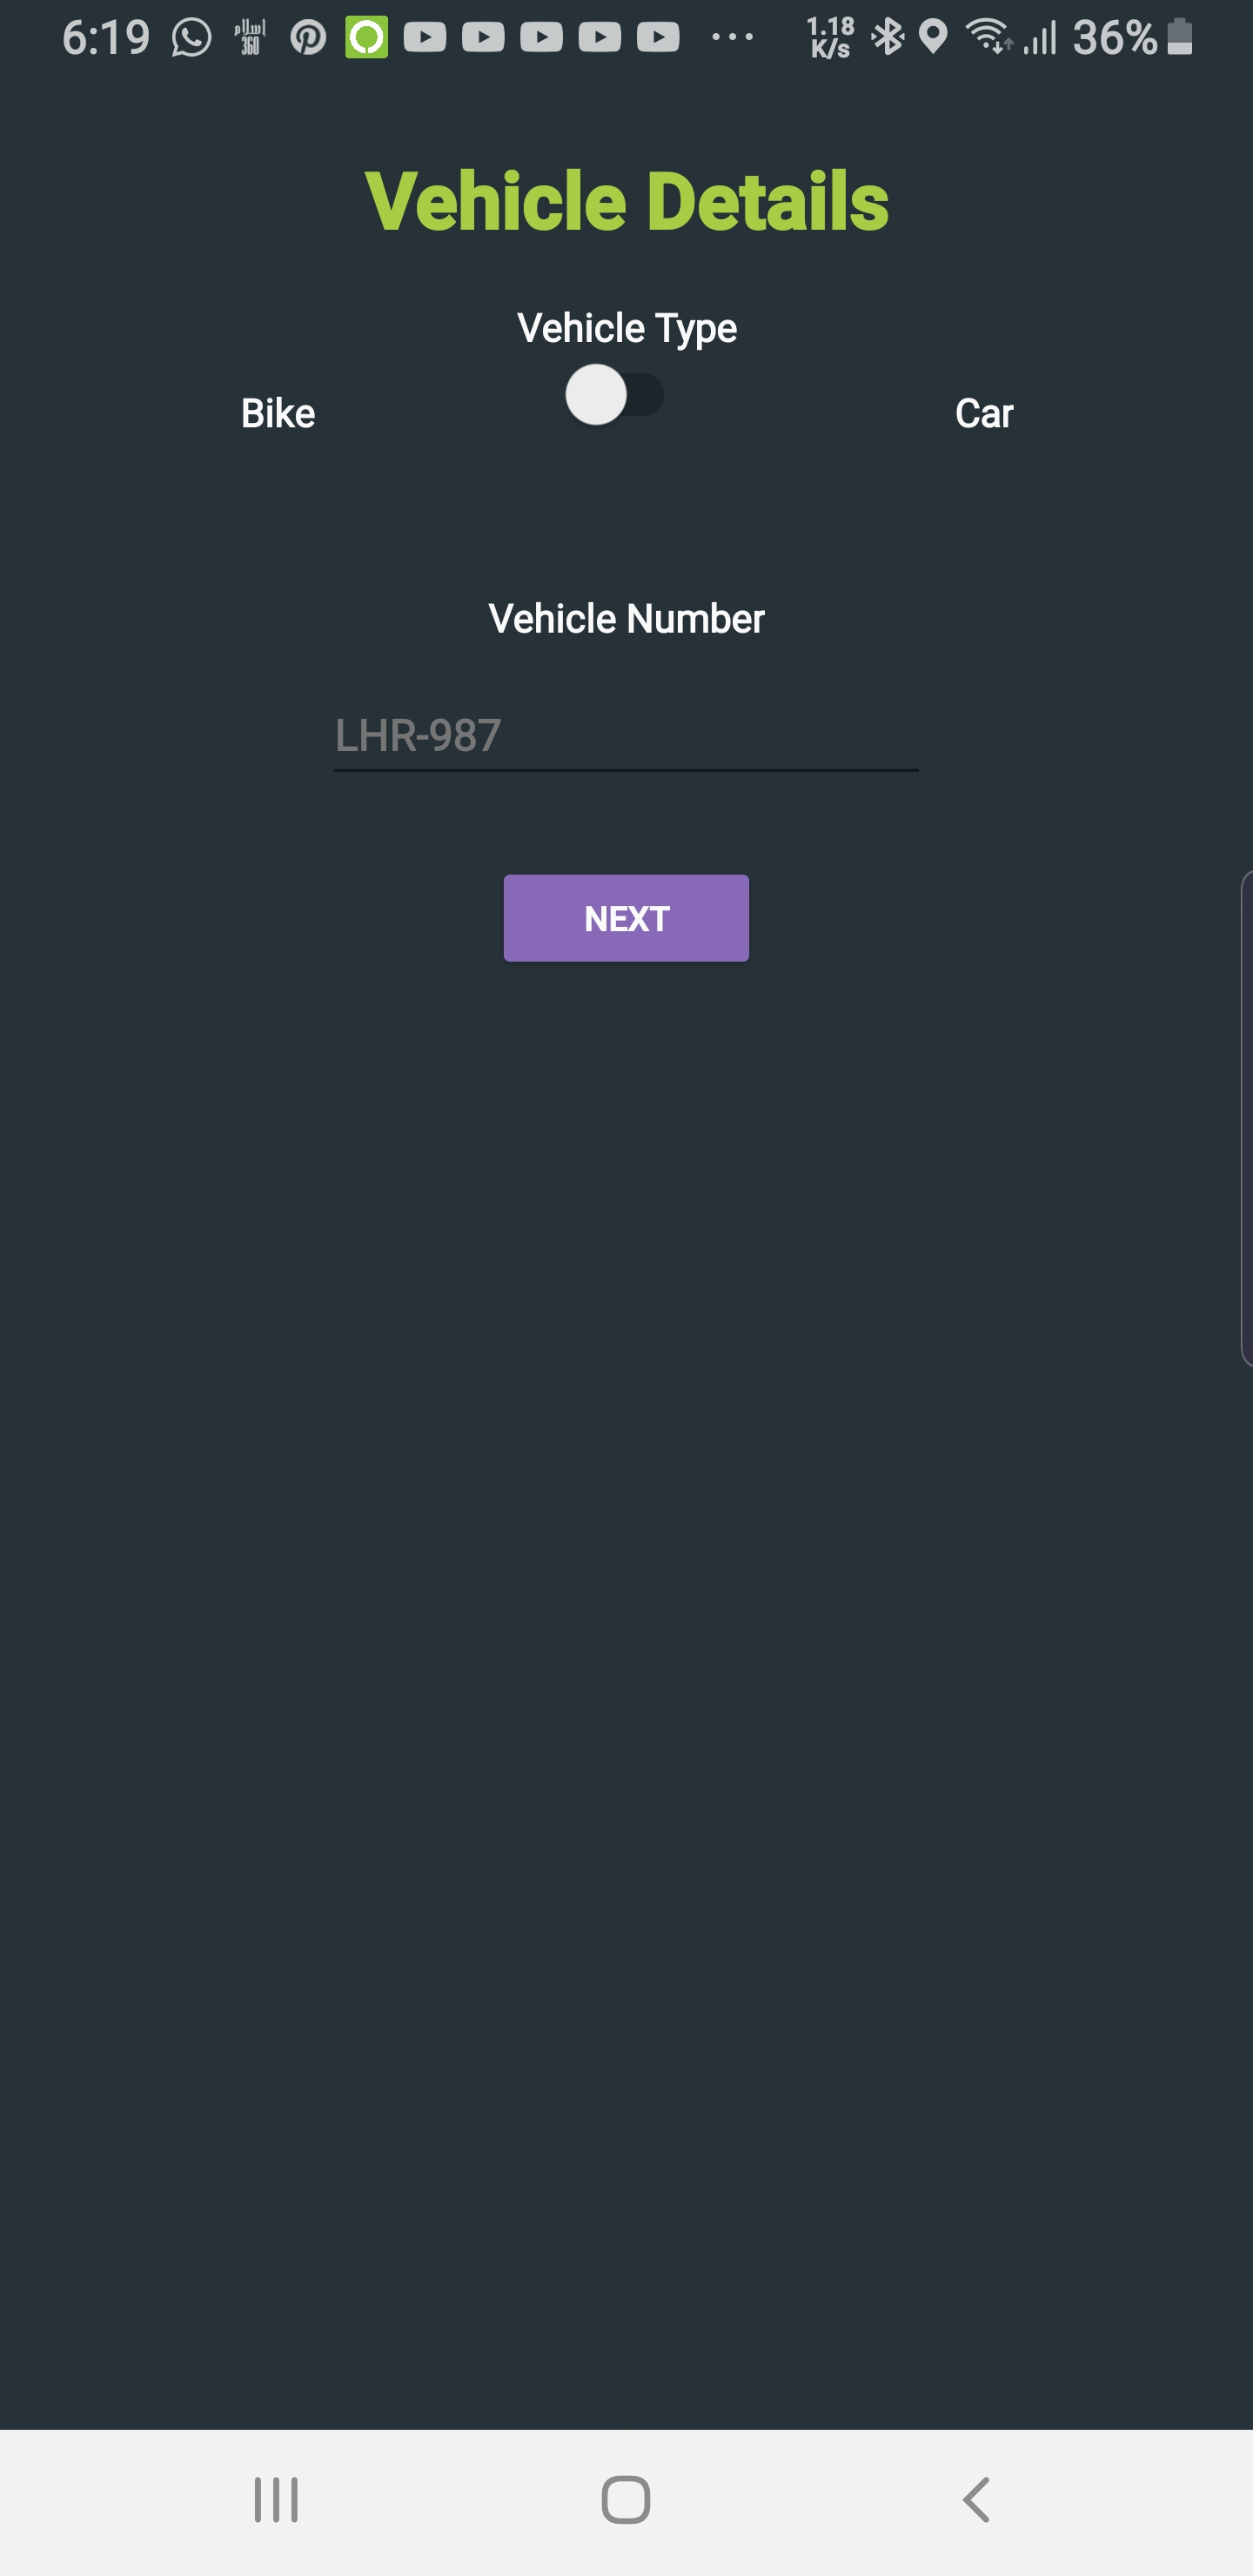
\includegraphics[width = 2in]{S10}}\hfill 
\subfloat[Driver Map Screen]{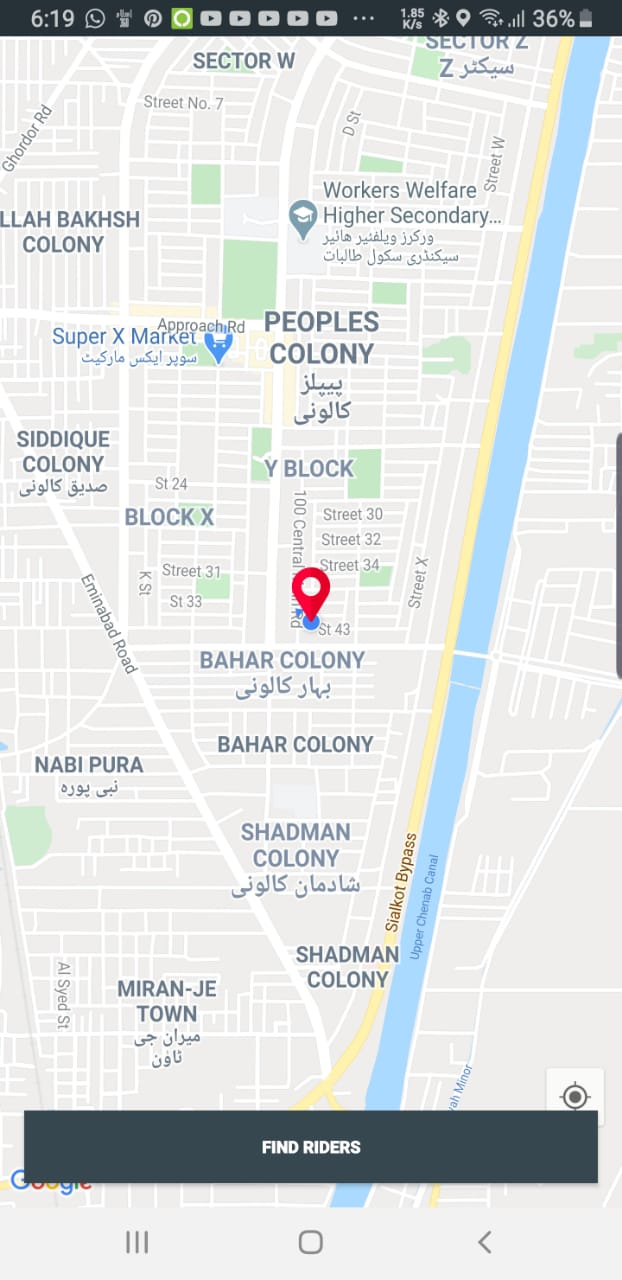
\includegraphics[width = 2in]{S11}}
\hspace*{\fill}\\
\hspace*{\fill}
\subfloat[Rider List Screen]{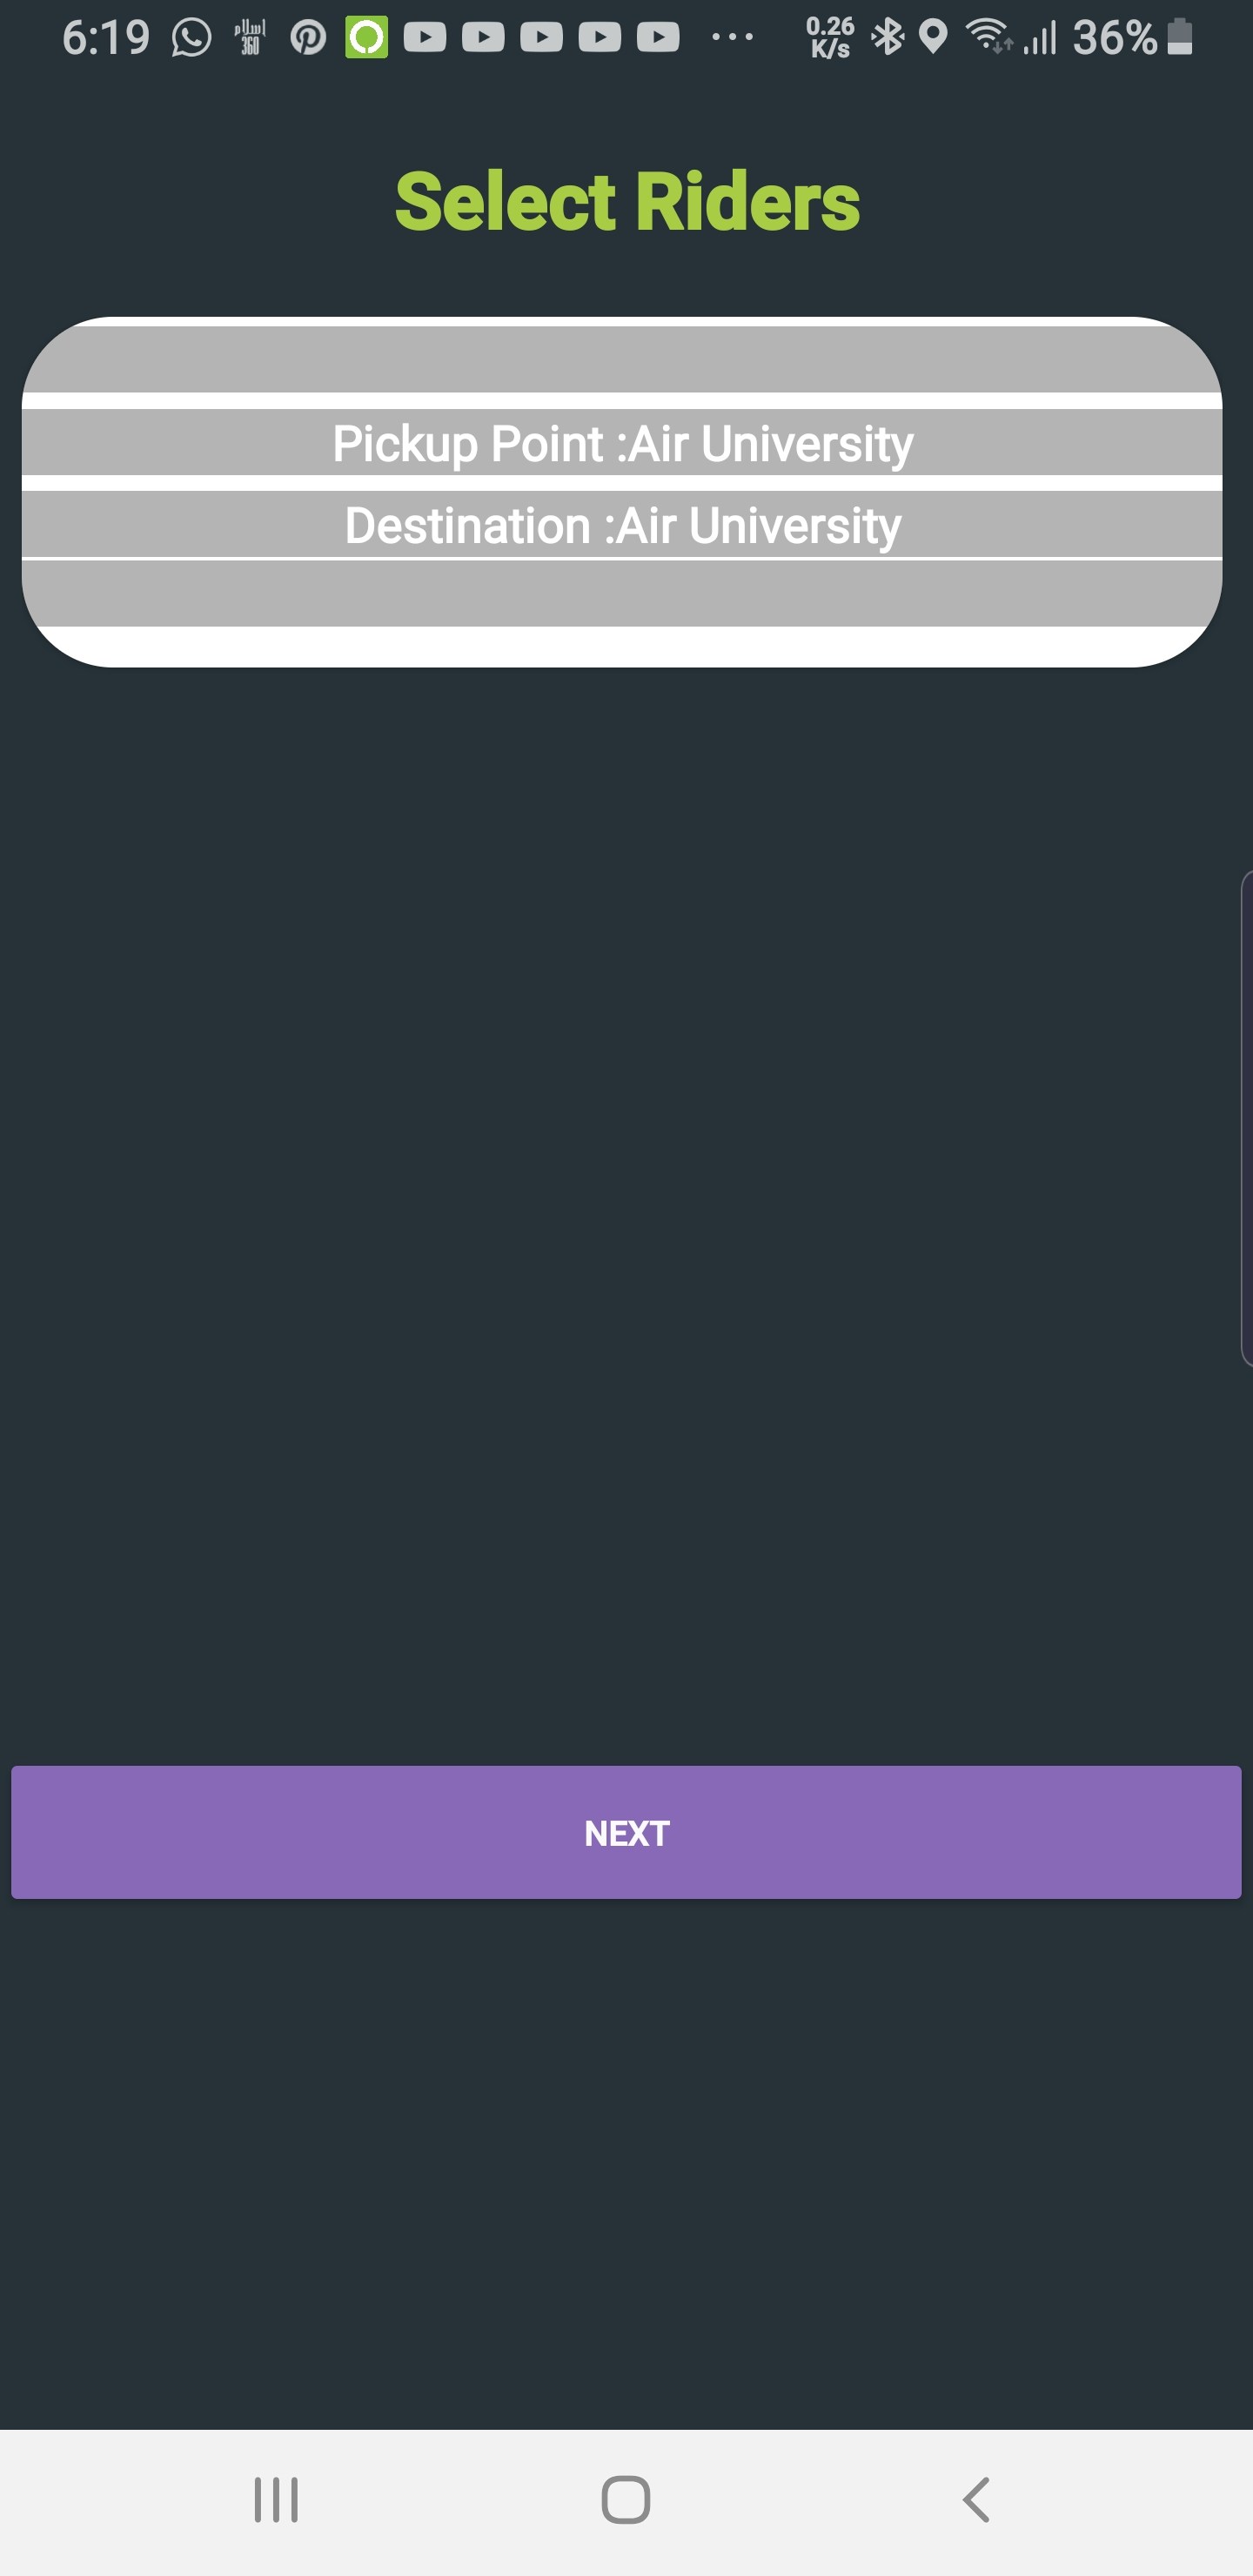
\includegraphics[width = 2in]{S12}}\hfill 
\subfloat[Popup Selection Confirmation Screen]{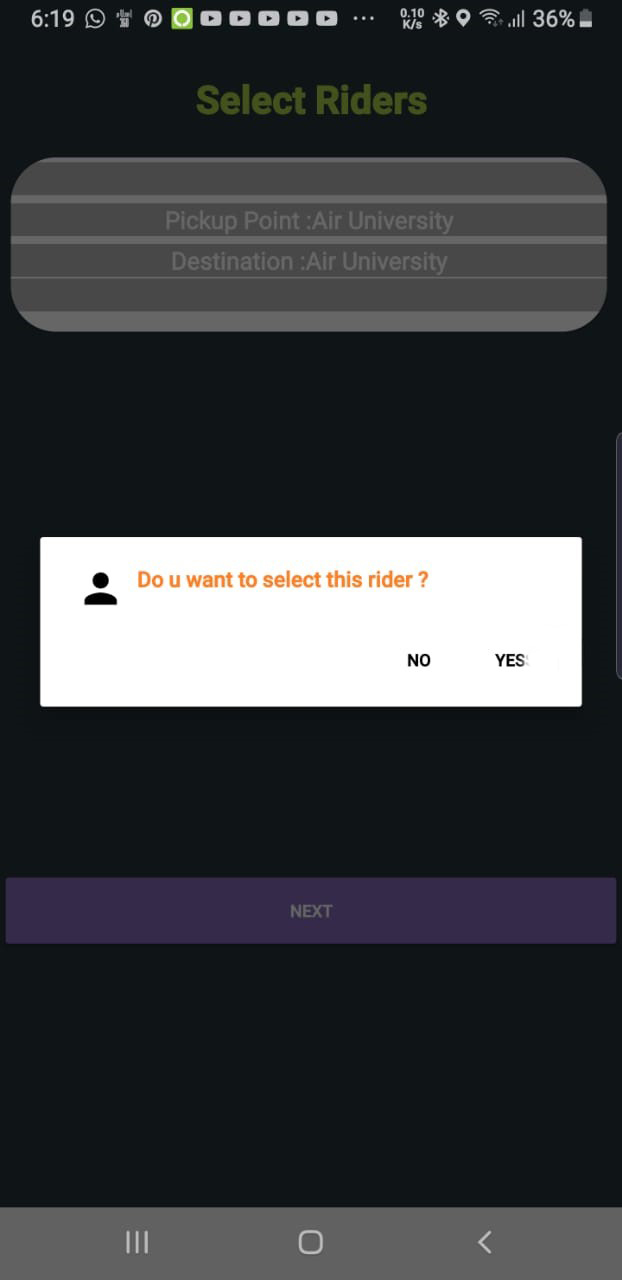
\includegraphics[width = 2in]{S13}}
\hspace*{\fill}
\end{figure}

\begin{figure}
\hspace*{\fill}
\subfloat[Selected Passengers Screen]{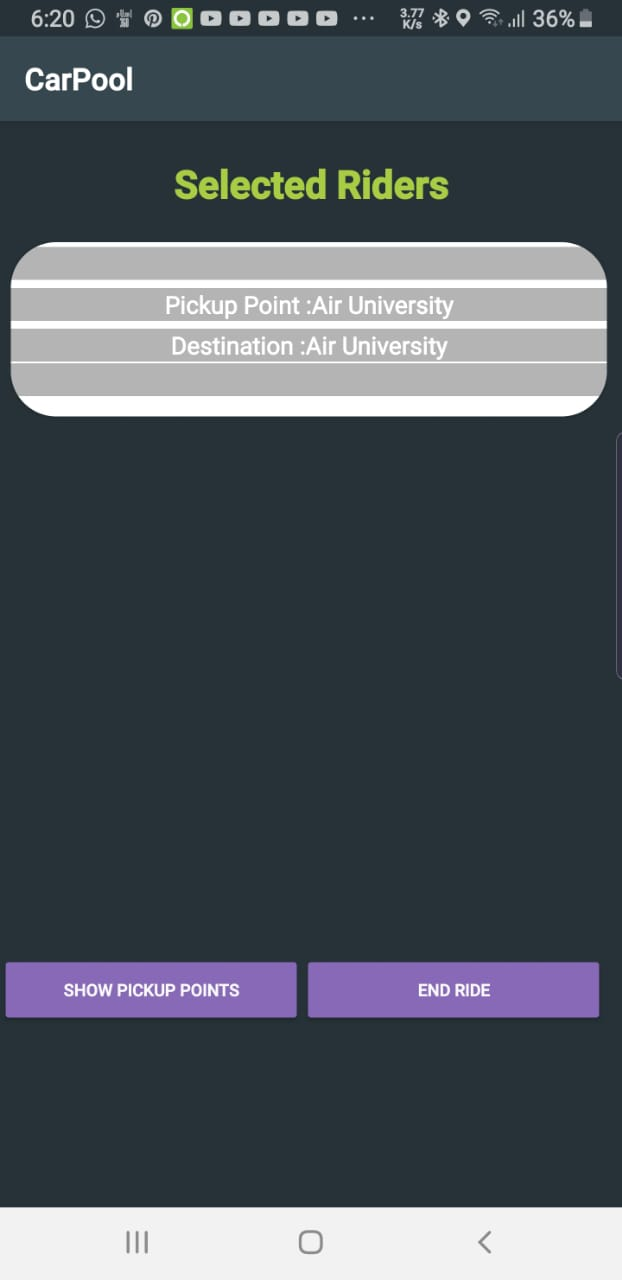
\includegraphics[width = 2in]{S14}}\hfill 
\subfloat[Passengers Pickup Points Screen]{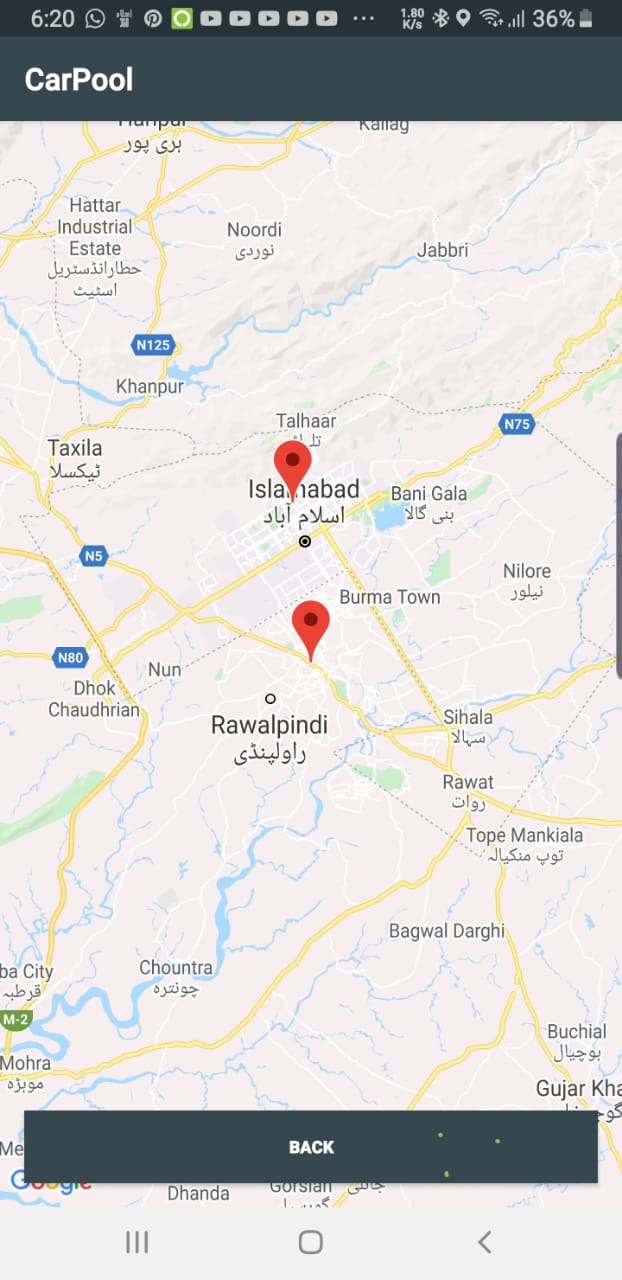
\includegraphics[width = 2in]{S15}}
\hspace*{\fill}
\end{figure}

\begin{figure}
\centering
\subfloat[Driver Summary Screen]{\includegraphics[width = 2in]{S16}}
\end{figure}
\chapter{System Implementation} \label{chap:sysImplementation}

\section{System Architecture}
Application architecture is a set of technologies and models for the development of 
fully-structured mobile programs based on industry and vendor-specific standards. As we develop the architecture of our application, we also consider programs that work on wireless devices such as smartphones and tablets.

\begin{figure}[ht]
\center
\includegraphics[width=0.8\textwidth]{SystemArchitectureCH5}
\caption{System Architecture}
\label{fig:System Architecture}
\end{figure}

\section{Work Environment}

\subsection{Hardware platforms}
For the development of this application we have used an Hp Elitebook workstation 8460w it fairly powerful and could handle the usage of multiple emulators at once. Full Specifications:

\begin{itemize}
\item \textbf{Processor} : Intel® Core™ i7-2630QM Processor (2.0 GHz, 6 MB L3 Cache)
\item \textbf{Memory }: 12GB 1333 MHz DDR3 SDRAM (2D)
\item \textbf{Graphics }: AMD FirePro™ M3900 w/1 GB gDDR3
\item \textbf{HDD Drive }: 1TB
\end{itemize}

For the testing of the application on a real device we have used an Android Phone Samsung Galaxy Note 8, Huawei  Mate 10 Pro

\subsection{Software platforms}
As for the software part of the work environment we have used several tools 
and frameworks alongside different versions of android.

\subsection{Work Tools}
\begin{itemize}
\item \textbf{Operating System }: Windows 
\item \textbf{IDE }: Android Studio 3.2.1
\item \textbf{Emulators }: Pixel 3 Android 9 / Nexus 5 Android 6
\item \textbf{Real Device OS}: Android 9 Pie (Samsung Galaxy Note 8)
\item \textbf{Backend Management}: Firebase Platform
\item \textbf{Places and Map Tools}: Google Cloud Platform
\end{itemize}
 

\subsection{Programming languages:} 
\begin{itemize}
\item \textbf{Application Programming }: Java\\
Motivation: Java code is inherently safer than Kotlin code because it 
prevents common programming mistakes by design, resulting in fewer 
system failures and application crashes. When using Kotlin, certain error 
causes are more likely to occur again.
\item \textbf{Layout Design }: XML
\item \textbf{Database Language }: NoSQL
\end{itemize}

\subsection{Frameworks used:}
\begin{itemize}
\item \textbf{Firebase Auth }: this framework that lets you implement easy Authentication in thisapplication email and phone number authentication was used.
\item \textbf{Firebase Real-time Database }: this framework is used as our main Database for 
this application it lets you read and write data from firebase in a NoSQL structure. 
\item \textbf{Firebase Storage }: this framework is used to upload and download data such as 
photos and videos, this is used to store user pictures for our database.
\item \textbf{Firebase Messaging }: a framework that makes real time messaging easy and possible using firebase, it’s also used for push notifications, this used for our messaging function between users in our application. 
\item \textbf{ Google Maps API }a great API used for MapView that enables the application to show places on the map like the origin and destination and the way between them, it’s used in the map to trace the destination on the map for users.
\item \textbf{Google Places API }: a very powerful API used to give information about places in the application and used to AutoComplete search queries, it’s used to autocomplete search queries for our users for easier searching, it’s also used to optimize our search function.
\item \textbf{Material Design Library }: material Design Library with all of its components such as Material Buttons, Material EditText etc.
\item \textbf{RuntimePermission }: a small library to help manage Android Permissions with no problems. 
\item \textbf{DxLoadingButton }: a small library with a loading button used for Authentication. 
\item \textbf{StfalconImageViewer }: a simple and customizable Android full-screen image viewer with shared image transition support, "pinch to zoom" and "swipe to dismiss" gestures.
\item \textbf{Spinner }: A styleable drop down menu for Android using the old spinner style. 
\item \textbf{Tooltip }: Simple to use customizable Android Tooltips library based on PopupWindow. 
\item \textbf{EasyValidation }: A text and input validation library in Java for Android. Used to validate user input info.
\item \textbf{Retrofit }: Type-safe HTTP for Android and Java.
\end{itemize}

\section{Database Management System}
To manage the backend of our application we decided to use Firebase Real-time Database alongside with Firebase Auth and Firebase Storage. 
\begin{itemize}
\item \textbf{Firebase Real-time Database }\\
it’s a database structured in a NoSQL way, it’s usage is very easy and very fast, we have used this database to store User objects which contain all the information about the user such as name, email, number etc., we have also used it to store Trip and TripRequest objects .
\textbf{example of the user node in the database}
\end{itemize}
\begin{figure}[ht]
\center
\includegraphics[width=1.2\textwidth]{DB} 
\caption{Example of a user mode in database}
\label{fig:Example of a user mode in database}
\end{figure}

\begin{itemize}
\item \textbf{Real-time Database Usage }\\
For the usage of this Database a separate Database class was made on Java this 
class contains all Database related functions the functions require a listener interface that 
has \textbf{onStart(), onSuccess(), onFailed(),} the interface is used to listen to changes in other 
classes.
\\ The reason for creating a separate class with a listener interface is to make 
migration to another Database easier. If we ever decide to switch to another database we 
will only change the content of the Database class which would make changes faster, more 
professional and effective. 
\\ Firebase’s Real-time Database allows you to use different query methods 
to fetch data from its Database: 
\\ The first method is using \textbf{addListenerForSingleValueEvent,} this method listens to changes 
in data for one time and does not trigger until it’s called again, this is good for fetching data 
only once. 
\\ The second method is using \textbf{addValueEventListener,} this method listens 
to data every time it changes and it also triggers every time it changes this is 
good for things like messages and real time updates. 
In our real. 
\\ We have decided to use \textbf{addListenerForSingleValueEvent} for most of our data 
fetching, the reason is each time data has been read, Firebase charges for it, which means 
it the less data is fetched the better, for this we have avoided using\textbf{ addValueEventListener} 
Instead we fetch the data once and save it locally, when the data is changed the user is 
required to refresh the page to get updates. However in cases where it’s important to get 
updates in real time like in messages we have used \textbf{addValueEventListener}. 
\end{itemize}

\section{Tools and Technology}
\begin{itemize}
\item Android
\item Firebase Platform
\item Google Cloud Platform
\item Android Studio
\item Java Language
\item Google Maps API
\item Google Direction API
\item Google Places API
\end{itemize}

\section{System requirements}
\begin{itemize}
\item Android phone with Minimum SDK android API 19 Kit Kat 
\item Google Play Services
\item GPS service
\item Internet Connection
\end{itemize}

\section{Security}
\begin{itemize}
\item \textbf{Firebase Authentication}\\ 
Firebase Authentication is a very fast and secure way to sign users into our application it is used to Login and Register users into our database in our case we are using the email verification, a user must verify his email to complete the registration.
\item \textbf{Authentication Usage}\\
When a user registers, his basic information (Name, Email, Password) are registered in the Auth Database but not the RealTime Database, after that users are welcomed with a finish registration activity, in this activity they have to verify their email using EMAIL verification, this method is used to prevent spam and multiple account creations, after verification and filling other information user data is saved on the RealTime Database. As for the login the system checks data and logs users if it’s correct.
\end{itemize}

\section{Rules}
Some of the restriction and rules are mentioned below :
\begin{itemize}
\item User can be used one account for both driver and rider.
\item Users cannot modify anyone else’s data except theirs.
\item Only the admin can modify the data of other users.
\item The driver cannot select more than three riders.
\item The rider can only contact with their driver.
\item A rider have to select pick up and drop off points.
\item Driver, Rider cannot use the app until their accounts are verified.
\end{itemize}


 


 






\chapter{System Testing and Evaluation}\label{chap:testingEvaluation}

\section{Graphical user interface testing}
\begin{figure}[ht]
\subsubsection{Table 28: user interface testing}
\centering
\includegraphics[width=0.8\textwidth]{UITesting1}
\captionof{table}{User Interface Testing}
\end{figure}

\section{Graphical user interface testing}
\begin{figure}[ht]
\subsubsection{Usability testing}
\centering
\includegraphics[width=0.8\textwidth]{UsabilityTesting1}
\includegraphics[width=0.8\textwidth]{UsabilityTesting2}
\captionof{table}{Usability Testing}
\end{figure}

\begin{figure}
\centering
\includegraphics[width=0.8\textwidth]{UsabilityTesting3}
\end{figure}

\begin{figure}
\section{Software performance testing}
\subsubsection{user interface testing}
\centering
\includegraphics[width=0.8\textwidth]{PFTesting}
\captionof{table}{Software Performance Testing}
\end{figure}

\begin{figure}
\section{Compatibility testing}
\subsubsection{Compatibility testing}
\centering
\includegraphics[width=0.8\textwidth]{CompatibilityTesting}
\captionof{table}{Compatibility testing}
\end{figure}

\begin{figure}
\section{Exception handling}
\subsubsection{Exception handling}
\centering
\includegraphics[width=0.8\textwidth]{EHTesting}
\captionof{table}{Exception Handling}
\end{figure}

\begin{figure}
\section{Security testing}
\subsubsection{Security testing}
\centering
\includegraphics[width=0.8\textwidth]{SecurityTesting}
\captionof{table}{Security Testing}
\end{figure}

\begin{figure}[t]
\section{Installation testing}
\subsubsection{Installation testing}
\centering
\includegraphics[width=0.8\textwidth]{InstallationTesting}
\captionof{table}{Installation Testing}
\end{figure}



\chapter{Conclusions and Future Work}\label{chap:conclusions}

The implementation from a concept to a real application was extremely challenging but it was very effective and full of experience. The final application turned out to be very professional and organized. It contained all necessary features to make both the driver and the passenger feel comfortable using it. From design to backend features, everything is checked. After a lot of testing and bug fixes the application finally reached a final state with no known bugs.\\

We have implemented all functional and non-functional needs and some of the optional needs. Some additional features were added to make the application more usable but the core concept stayed the same. Since it offers all the mentioned features and needs in the project description. It also respects the optimization needs such as good code design style, small sized application(4mb) and targeting as many android devices as possible.\\

By using Java which is the official programming language for android, we have made sure that the code was well structured as well as optimized. Since android itself is built on Java, there are plenty of Java libraries available and Java has a wide open-source ecosystem. Java apps are lighter even when compared to Kotlin apps, resulting in a faster app experience. Java yields a faster build process too, letting you code more in less time. Thanks to the accelerated assembly with gradle due to which assembling large projects becomes easier in Java.\\

As for the backend is concerned, our best choice was Firebase because it’s very powerful and simple to use, especially for beginners. It also contains a free usage tier with good performance. The application does its best to optimize the backend for both database usage and user experience. Firebase provided all necessary backend functions which helped making a professional application on time.\\
 
By using all the tools and libraries available and all knowledge of data structures and object-oriented programming, we were able to make a well-designed application that could be used without bugs and didn’t lack any important features. This implementation was definitely helpful to our career, since implementing a concept into a real application gives us good knowledge of the development environment.\\

Now that the application has been developed, we can look back and tell how much we have learned from this project. So many things could have been done differently, in terms of implementation and design concept also. Many additional features that an application like this could have to be more useful and competitive.\\

When the application was first being designed there were so many concerns that were not considered. By the time of developing and testing the application, we have realized so many things in terms of design and code optimization. Because of this, we modified so many things since we started working on the implementation just to make sure that application is more efficient and optimized. This proves that working on this project made us learn so many things about software development in general. Not only this, we also learned how to make better conceptual design and learned how to turn an idea into a real application.\\

There are some ways in which this application can be improved further. Some of the features for the application which are not yet present, but could be implemented in future development.\\

Our group has primarily been focusing on the functionality and simplicity of this application. If time allows, we we'll try to make the GUI more colourful and elegant, but there'll always be room for betterment in this segment.
\appendix
\chapter{Application Workflow} \label{ap:Appendix1}

\section*{}
The user downloads and installs the application in an android device. The user opens the application then he is welcomed with a Login/Register. New user register via the register form (name, university email, university registration id, contact no, password). The user must have to confirm the registration via email.\\

After confirmation the user enters the application and chooses between driver/rider if the user is a driver he can enter vehicle detail and select riders from list of passengers.\\

Riders can enter trip details and request a ride, after selected by driver display the details of driver to passenger.\\

After completion of ride both driver and rider can see the summary of ride.


\chapter{Interviews} \label{ap:Appendix1}

\section*{}
The interviewees were three students from different departments of Air University.\\~\\
\large {\textbf{Student 1 }}
\\ Name : Hassan Siddiqui 
\\ Age : 21 
\\ Sex : Male
\\ Interview date : 10.02.2020 
\\ Duration of interview : 10 minutes 
\\ Place of interview : AUSOM building 
\\ Method : Note taking and no recording as we believe recording would make interviewees uncomfortable.
\\ Notes from interview : The interviewee owns a Samsng Galaxy S9 smart-phone which runs android 9.0, he is not familiar with concept of programming for mobile devices but he believes it is a very interesting concept. Hassan believes our app is very handy and he would even liked to install our prototype, on his own smart-phone and become one of our test users. the interviewee would like easier access to travel to and from university he believes it is not easy to find out local transportation. he mentioned that he would be even happier that he can share their ride expenses and cut their fuel bills.\newpage
\large {\textbf{Student 2 }}
\\ Name : Ahmed Shahid
\\ Age : 29 
\\ Sex : Male
\\ Interview date : 10.02.2020 
\\ Duration of interview : 8 minutes 
\\ Place of interview : Department of Mechatronics
\\ Method : Note taking and no recording as we believe recording would make interviewees uncomfortable. \\\ Notes from interview : The interviewee owns a iPhone 7 smart-phone which runs IOS. he is not familiar with concept of programming for mobile devices but he believes it is a very interesting concept. Ahmed believes our app is very useful and he wishes a similar application for iPhone. The interviewee would like to use this application through cell phone, or his future iPad. he specially would like to share ride with non-vehicle owning students.\\~\\
\large{\textbf{Student 3}} 
\\ Nickname : Amna Asim 
\\ Age : 19 
\\ Sex : Female 
\\ Interview date : 10.02.2020 
\\ Place of interview : Department of Electrical Engineering
\\ Duration of interview : 5 minutes 
\\ Method : Note taking and no recording as we believe recording would make interviewees uncomfortable.
\\ Notes from interview : The interviewee owns a Oppo K1 smart-phone which runs Android 8.1. she is not familiar with concept of programming for mobile devices and she believes it is a very interesting that someone finally is doing this for students. she complained a lot about the local transportation in Islamabad which frustrate her every time she wants to travel to and from university. she believes also that it is a good idea to share ride with other non-vehicle owning students. she also mention that include the feature that facilitate female students to share ride with only female students.
 
\chapter{Steeple Analysis} \label{ap:Appendix1}

\section*{Social}
\begin{itemize}
\item Increase social interaction and solidarity.
\item Meet new people during rides and make new friends.
\item Driving with people is better than driving alone since it involves less stress.
\end{itemize}

\section*{Technology}
\begin{itemize}
\item Smartphone penetration is increasing day after day.  
\item Use of technology to create matches between drivers and passengers.
\item The application is accessible from anywhere using a smartphone  real time communication between actors.
\end{itemize}

\section*{Environmental}
\begin{itemize}
\item Increase of high occupancy vehicles which will lead to a decrease of CO2 emissions.
\item Less cars on the roads that leads to safer roads and fluent traffic. 
\end{itemize}

\section*{Economical}
\begin{itemize}
\item Savings as the price of gas and highways is shared among the travelers in a context of an increasing gas price.
\end{itemize}

\section*{Political}
\begin{itemize}
\item Increase of support for initiatives that decreases greenhouse gas emission support from government thank to the benefits of carpooling.
\end{itemize}

\section*{Legal}
\begin{itemize}
\item Insurances of drivers and passengers: In case of accidents, if the owner of the car have insurance it covers any medical expense. Carpool more than other racial and ethnic groups.
\item Ride sharing serves an important role in enhancing mobility in low-income, hostel students who are more likely to be unable to afford personal automobiles.
\end{itemize}

\section*{Ethical}
\begin{itemize}
\item Client confidentiality should be kept: all information related to trips’ history should only be communicated to their respective use.
\end{itemize} 
  

\begin{thebibliography}{9}
\bibitem{latexcompanion} 
Michel Goossens, Frank Mittelbach, and Alexander Samarin. 
\textit{The \LaTeX\ Companion}. 
Addison-Wesley, Reading, Massachusetts, 1993.

\bibitem{einstein} 
Albert Einstein. 
\textit{Zur Elektrodynamik bewegter K{\"o}rper}. (German) 
[\textit{On the electrodynamics of moving bodies}]. 
Annalen der Physik, 322(10):891–921, 1905.

\bibitem{knuthwebsite} 
Knuth: Computers and Typesetting,
\\\texttt{http://www-cs-faculty.stanford.edu/\~{}uno/abcde.html}
\end{thebibliography}

\end{document}